\documentclass[a4paper, 12pt]{article}

\usepackage{cmap} % поиск в PDF
\usepackage[english, russian]{babel} % локализация и переносы
\parskip=3pt % дополнительное расстояние между абзацами
\usepackage{graphicx} % вставка рисунков
\usepackage{lastpage}
\usepackage{rotating}
%\usepackage{minted} % красивый код
%\usemintedstyle{friendly}

\usepackage{verbatim}
\usepackage{multirow} % Слияние строк в таблице
\usepackage{caption}
\usepackage{amsfonts, amssymb, amsthm, mathtools, amsmath} % AMS
\usepackage{array} % Дополнительная работа с таблицами
\usepackage{multicol}

%%% Цветной текст

\usepackage[usenames]{color}
\usepackage{colortbl}

%% Поля

\usepackage{geometry} 
\geometry{left=2cm}
\geometry{right=2cm}
\geometry{top=2cm}
\geometry{bottom=2cm}

%%% Гиперссылки

\usepackage[unicode]{hyperref}
\usepackage{xcolor}
\definecolor{urlcolor}{HTML}{3E5F8A} % цвет гиперссылок
\definecolor{linkcolor}{HTML}{3E5F8A} % цвет ссылок
\definecolor{citecolor}{HTML}{3E5F8A} % цвет библиоссылок
\hypersetup{pdfstartview=FitH,  linkcolor=linkcolor,urlcolor=urlcolor, citecolor=citecolor, colorlinks=true}

%% Немного дизайна

\definecolor{lb}{rgb}{0.8,0.85,1}
\renewcommand{\labelitemi}{$\diamond$}

\newcommand{\e}{\mathbb{E}}
\newcommand{\p}{\mathbb{P}}
\newcommand{\n}{\mathbb{N}}
\newcommand{\id}{\mathbb{I}}
\newcommand{\re}{\mathbb{R}}
\DeclareMathOperator{\plim}{plim}
\DeclareMathOperator{\var}{Var}
\DeclareMathOperator{\svar}{sVar}
\DeclareMathOperator{\argmin}{argmin}
\renewcommand{\epsilon}{\varepsilon}
\newcommand{\msum}{\sum\limits_1^n}
\newcommand{\isum}{\sum\limits_i^n}
\newcommand{\jsum}{\sum\limits_j^n}

\newcommand{\ds}{\displaystyle}

\begin{document}

\thispagestyle{empty}
\begin{center}
	\textbf{ПРАВИТЕЛЬСТВО РОССИЙСКОЙ ФЕДЕРАЦИИ}\\
	\vspace{3ex}
	\textbf{Федеральное государственное автономное\\ образовательное учреждение высшего образования}
	
	\vspace{3ex}
	
	\textbf{Национальный исследовательский университет \\ <<Высшая школа экономики>>}
	
	\vspace{10ex}
	\begin{flushright}
		Факультет экономических наук\\
		Образовательная программа <<Экономика>>
	\end{flushright}
\end{center}
\vspace{12ex}

\begin{center}
	{\textbf{КУРСОВАЯ РАБОТА
	}}
	\vspace{1ex}
	
	<<Методы интерпретации моделей машинного обучения>>
\end{center}
\vspace{4ex}
\begin{flushright}
	\noindent
	Студентка группы БЭК171\\Махнева Елизавета Александровна\\
	\vspace{13ex}
	Научный руководитель:\\
	Соколов Евгений Андреевич
	
\end{flushright}	

\vfill

\begin{center}
	Москва 2020
	
\end{center}
\newpage
	\tableofcontents
	\newpage
	
	\section{Введение}
	Во введении я хочу сказать про то что существует интерпретируемые и нет модели. Про то что нам хотелось бы интерпретировать и привести аргументы за (как минимум те 3 из презенташки). Наверное стоит объединить с блоком интерпретации, так как здесь особо больше нечего писать (если только много не получится), а воду лить не хочется

1. Интерпретируемые и нет модели. Желательно показать примеры, почему не интерпретируются.
2. Интерпретация нужна! Потому что...
3. Плюсы интерпретации и небольшие минусы
4. Что и как хотелось бы интерпретировать. Основы интерпретации -- какой она должна быть
5. Кратко перечислить методы, сказать какие они бывают
	\newpage
	
	\section{Методы интерпретации}
	\subsection{PDP}
	\textbf{PDP (Partial Dependence Plot, график частичной зависимости)} -- график, который показывает зависимость прогноза модели от значения отдельного признака. С его помощью мы можем понять, как некоторый признак влияет на предсказание. Данный график можно изобразить для двух либо трех признаков из имеющихся.

\subsubsection{Идея}
Визуализация -- это отличный способ интерпретации. Если мы хотим понять, как признаки влияют на результат, можно посмотреть, как меняется прогноз от изменения одного признака при прочих равных. В идеальной ситуации мы бы построили график зависимости результата от всех признаков и меняли бы только один. Однако мы сталкиваемся с проблемой: если признаков больше двух, построить график не получится. Поэтому чтобы сохранить возможность визуализации, можно анализировать зависимость результата от одного признака без учета влияния остальных, построив график зависимости от одного признака. Аналогично можно изучать влияние одновременно двух признаков, построив трехмерный график.

\underline{Пример PDP для одного признака} \cite{pdpgit}
\vspace{-7mm}

\begin{figure}[h]
	\centering{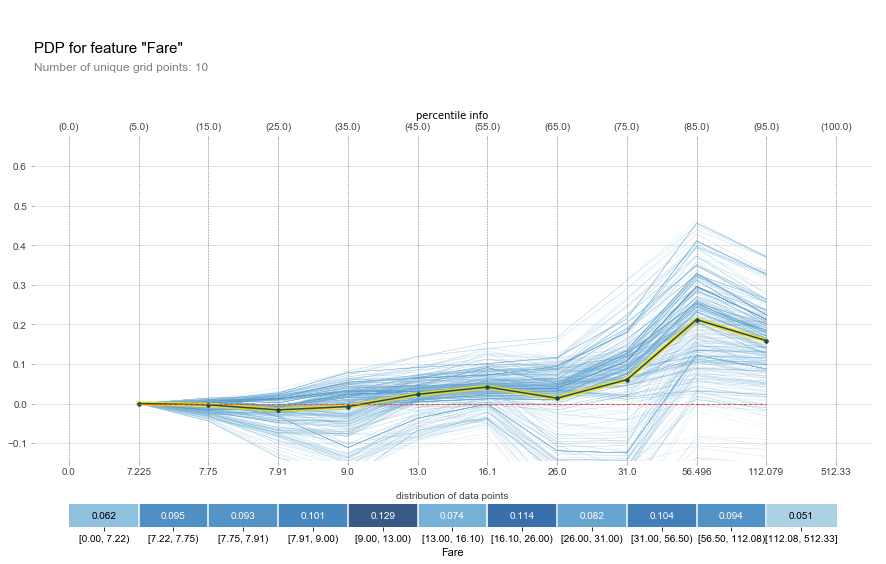
\includegraphics[width=0.95\linewidth]{pics/pdp1.png}}
\end{figure}

Желтая линия показывает, как в среднем выбранный признак <<Fare>> влияет на предсказание. Для упрощения визуализации значения признака по всем объектам были разбиты по квантилям -- так график для непрерывного признака становится более наглядным. По оси ординат указан непосредственно эффект признака: значение <<-0.1>> указывает на то, что признак уменьшает итоговое предсказание на 0.1. То есть данный график показывает <<предельный эффект>> признака. В данном случае можно сделать вывод, что <<Fare>> незначительно влияет при маленьких значениях признака. Но при возрастании начинает вносить ощутимый вклад в предсказание -- и зависимость при этом скорее положительная, но нелинейная.

\underline{Примеры PDP для двух признаков} \cite{pdpgit}
\vspace{-3mm}

\begin{figure}[h]
	\centering{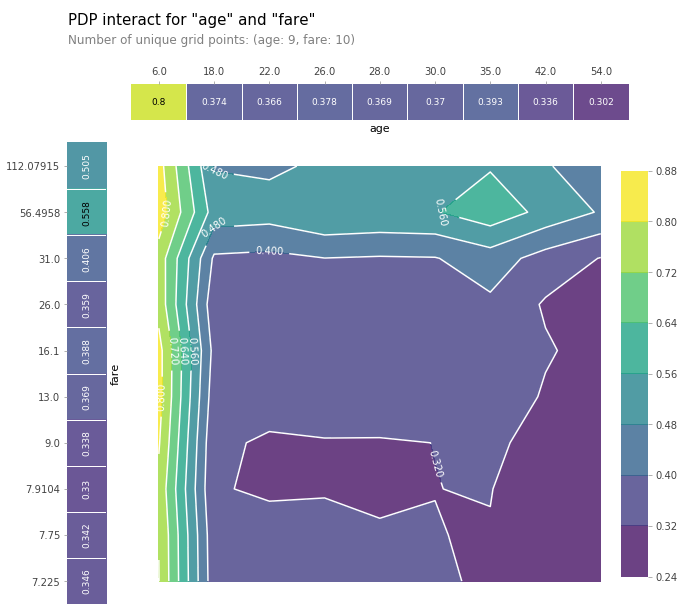
\includegraphics[width=0.75\linewidth]{pics/pdp2.png}}
\end{figure}
\vspace{-5mm}
\begin{figure}[h!]
	\centering{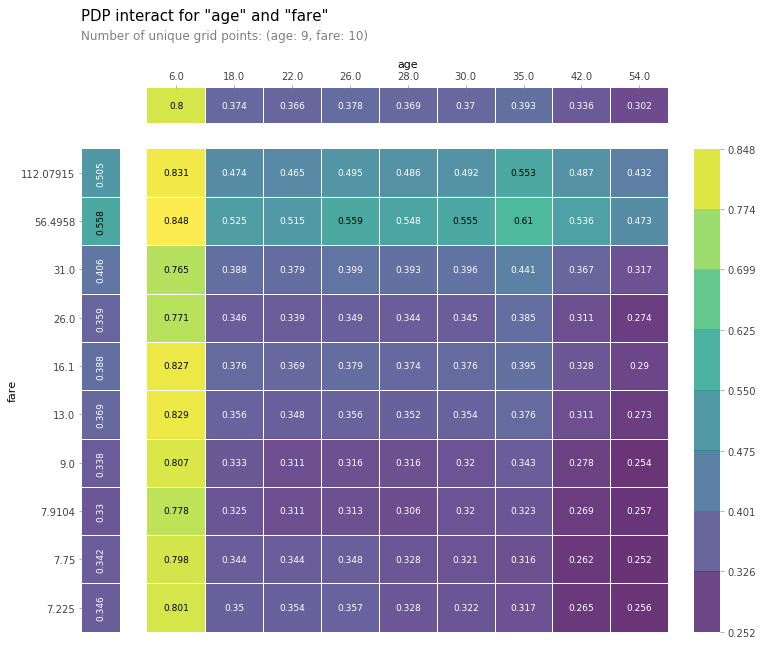
\includegraphics[width=0.76\linewidth]{pics/pdp3.png}}
\end{figure}

Отличие данных графиков от предыдущего заключается в том, что он показывает не предельные эффекты, а непосредственно предсказания модели. Первый график показывает линии уровня получившейся функции двух аргументов. Второй -- упрощенное представление линий уровня в виде сетки. Шкалы над и слева от графика показывают влияние каждого признака по отдельности -- сжатое представление графика для одного признака. По обоим графикам видно, что наименьшее значение предсказания достигается, когда значение <<fare>> наименьшее, а <<age>> -- наибольшее. Также можно отметить экстремум функции, который достигается при <<fare>> $\approx 56.4958$ и <<age>> $\approx 35$ -- зависимость нелинейная от обоих аргументов.
	\subsubsection{Принцип работы}
	Пусть $x = (x_1, \ldots, x_d)$ -- вектор признаков объекта. У нас есть модель $f(x): \re^d \rightarrow \re$. Мы хотим понять, как признаки $x_1$ и $x_2$ влияют на предсказание модели. Обозначим $x_r = (x_3, \ldots, x_d)$ за вектор остальных признаков.

Нам нужно получить функцию зависимости предсказания от одного-двух признаков при зафиксированных остальных: $g(x_1, x_2) = f(x_1, x_2 | \, x_r)$. % не знаю насколько корректно
Но если $x_1$ и/или $x_2$ зависимы с признаками из $x_r$, то возникает проблема. При изменении анализируемого признака меняется и зависимый с ним, который мы не рассматриваем -- мы не сможем рассмотреть чистый предельный эффект одного признака, на него всегда будет наложен эффект другого предиктора. Поэтому одной из предпосылок метода является независимость исследуемых признаков от остальных \cite{pdp}.

Но даже с предпосылкой о независимости признаков функция $g(x_1, x_2)$ не будет показывать точный результат, так как предельные эффекты предикторов разные для разных объектов выборки. Поэтому мы рассмотрим, как влияют анализируемые признаки на среднее предсказание. То есть найдем матожидание предсказания модели при фиксированных исследуемых признаках (как констант с точки зрения матожидания) \cite{pdp}:

\[
\bar{g}(x_1, x_2) = \e(f(x_1, x_2, x_r) \, | x_r)
\]

Таким образом, мы получим функцию, которая показывает предельные эффекты признаков для среднего предсказания. Но чтобы найти матожидание, мы должны знать истинные распределения признаков. Поскольку нам недоступна данная информация, можно воспользоваться методом Монте-Карло, чтобы примерно оценить искомую функцию \cite{basis}:

\[
\hat{g}(x_1, x_2) = \frac{1}{n} \isum f(x_1, x_2, X_r^{(i)}),
\]
где $X_r^{(i)}$ -- $i$ строка матрицы $X_r$, содержащей признаки $x_r$ для всех объектов выборки.
% не уверена что все красиво и понятно

Результат: функция показывает, как исследуемые признаки в среднем влияют на результат работы модели. Мы можем построить ее график, чтобы более наглядно посмотреть на влияние предикторов на предсказание.% не уверена что в среднем -- корректная формулировка

% почему бы просто эту функцию не находить
% способ дает меньшую точность там, где зависимость можно было достать из модели
% можно делать анимацию, если нельзя рассмотреть все сразу :)
% Должна быть предпосылка не о независимости случайных величин, а о том, что производная по исследуемому признаку не зависит от других величин
	\subsubsection{Реализация}
	Реализации данных графиков есть в разных библиотеках: $\verb|pdpbox|$, $\verb|sklearn|$,\\ $\verb|(sklearn.inspection.plot_partial_dependence|$,\\ $\verb|sklearn.ensemble.partial_dependence.plot_partial_dependence)|$

Библиотека $\verb|pdpbox|$ предоставляет более аккуратное и более наглядное представление графиков. Инструкции по установке можно найти \href{https://github.com/SauceCat/PDPbox}{здесь}.
	\subsection{LIME}
	LIME (Local Interpretable Model-Agnostic Explanations) -- метод, показывающий вклад признаков в отдельное предсказание, работающий с любой моделью.
% нужен ли перевод

\subsubsection{Идея}
Результаты некоторых моделей легко интерпретировать. Например, в линейной регрессии можно посмотреть на веса. Они показывают, насколько изменится предсказание при изменении признаков. Так для каждого конкретного предсказания можно понять, почему модель выдала именно такой результат -- виден непосредственный вклад каждого признака.

Но не все модели легко интерпретировать. Например, некоторые архитектуры нейронных сетей. Они зачастую значительно превосходят линейные модели, но при этом сама структура модели представляет собой <<черный ящик>> -- непонятно, как именно модель сформировала предсказание, какие признаки сильнее повлияли на решение нейронной сети.

Идея состоит в том, чтобы перенести свойство интерпретируемости простых моделей на более сложные. Мы можем обучить интерпретируемую модель по выборке, где ответами являются предсказания сложной модели. В процессе обучения модель анализирует зависимости непосредственно между признаками и предсказаниями сложной модели. Тогда мы сможем интерпретировать результаты простой модели, которые являются аппроксимацией предсказаний сложной.\\[2mm]
\begin{minipage}{0.57\linewidth}
\indent Возникает проблема: сложная модель выявляет зависимости, которые, например, линейная модель может не уловить. Идея данного метода заключается в том, чтобы обучать более простую модель в некоторой окрестности исследуемого объекта, предполагая что на очень локальном уровне нет сложных зависимостей \cite{lime_dop}. Например, дифференцируемые функции можно линеаризовать в окрестности заданной точки -- можно использовать линейную модель на локальном уровне.
\end{minipage}
\hspace{5mm}
\begin{minipage}{0.35\linewidth}
	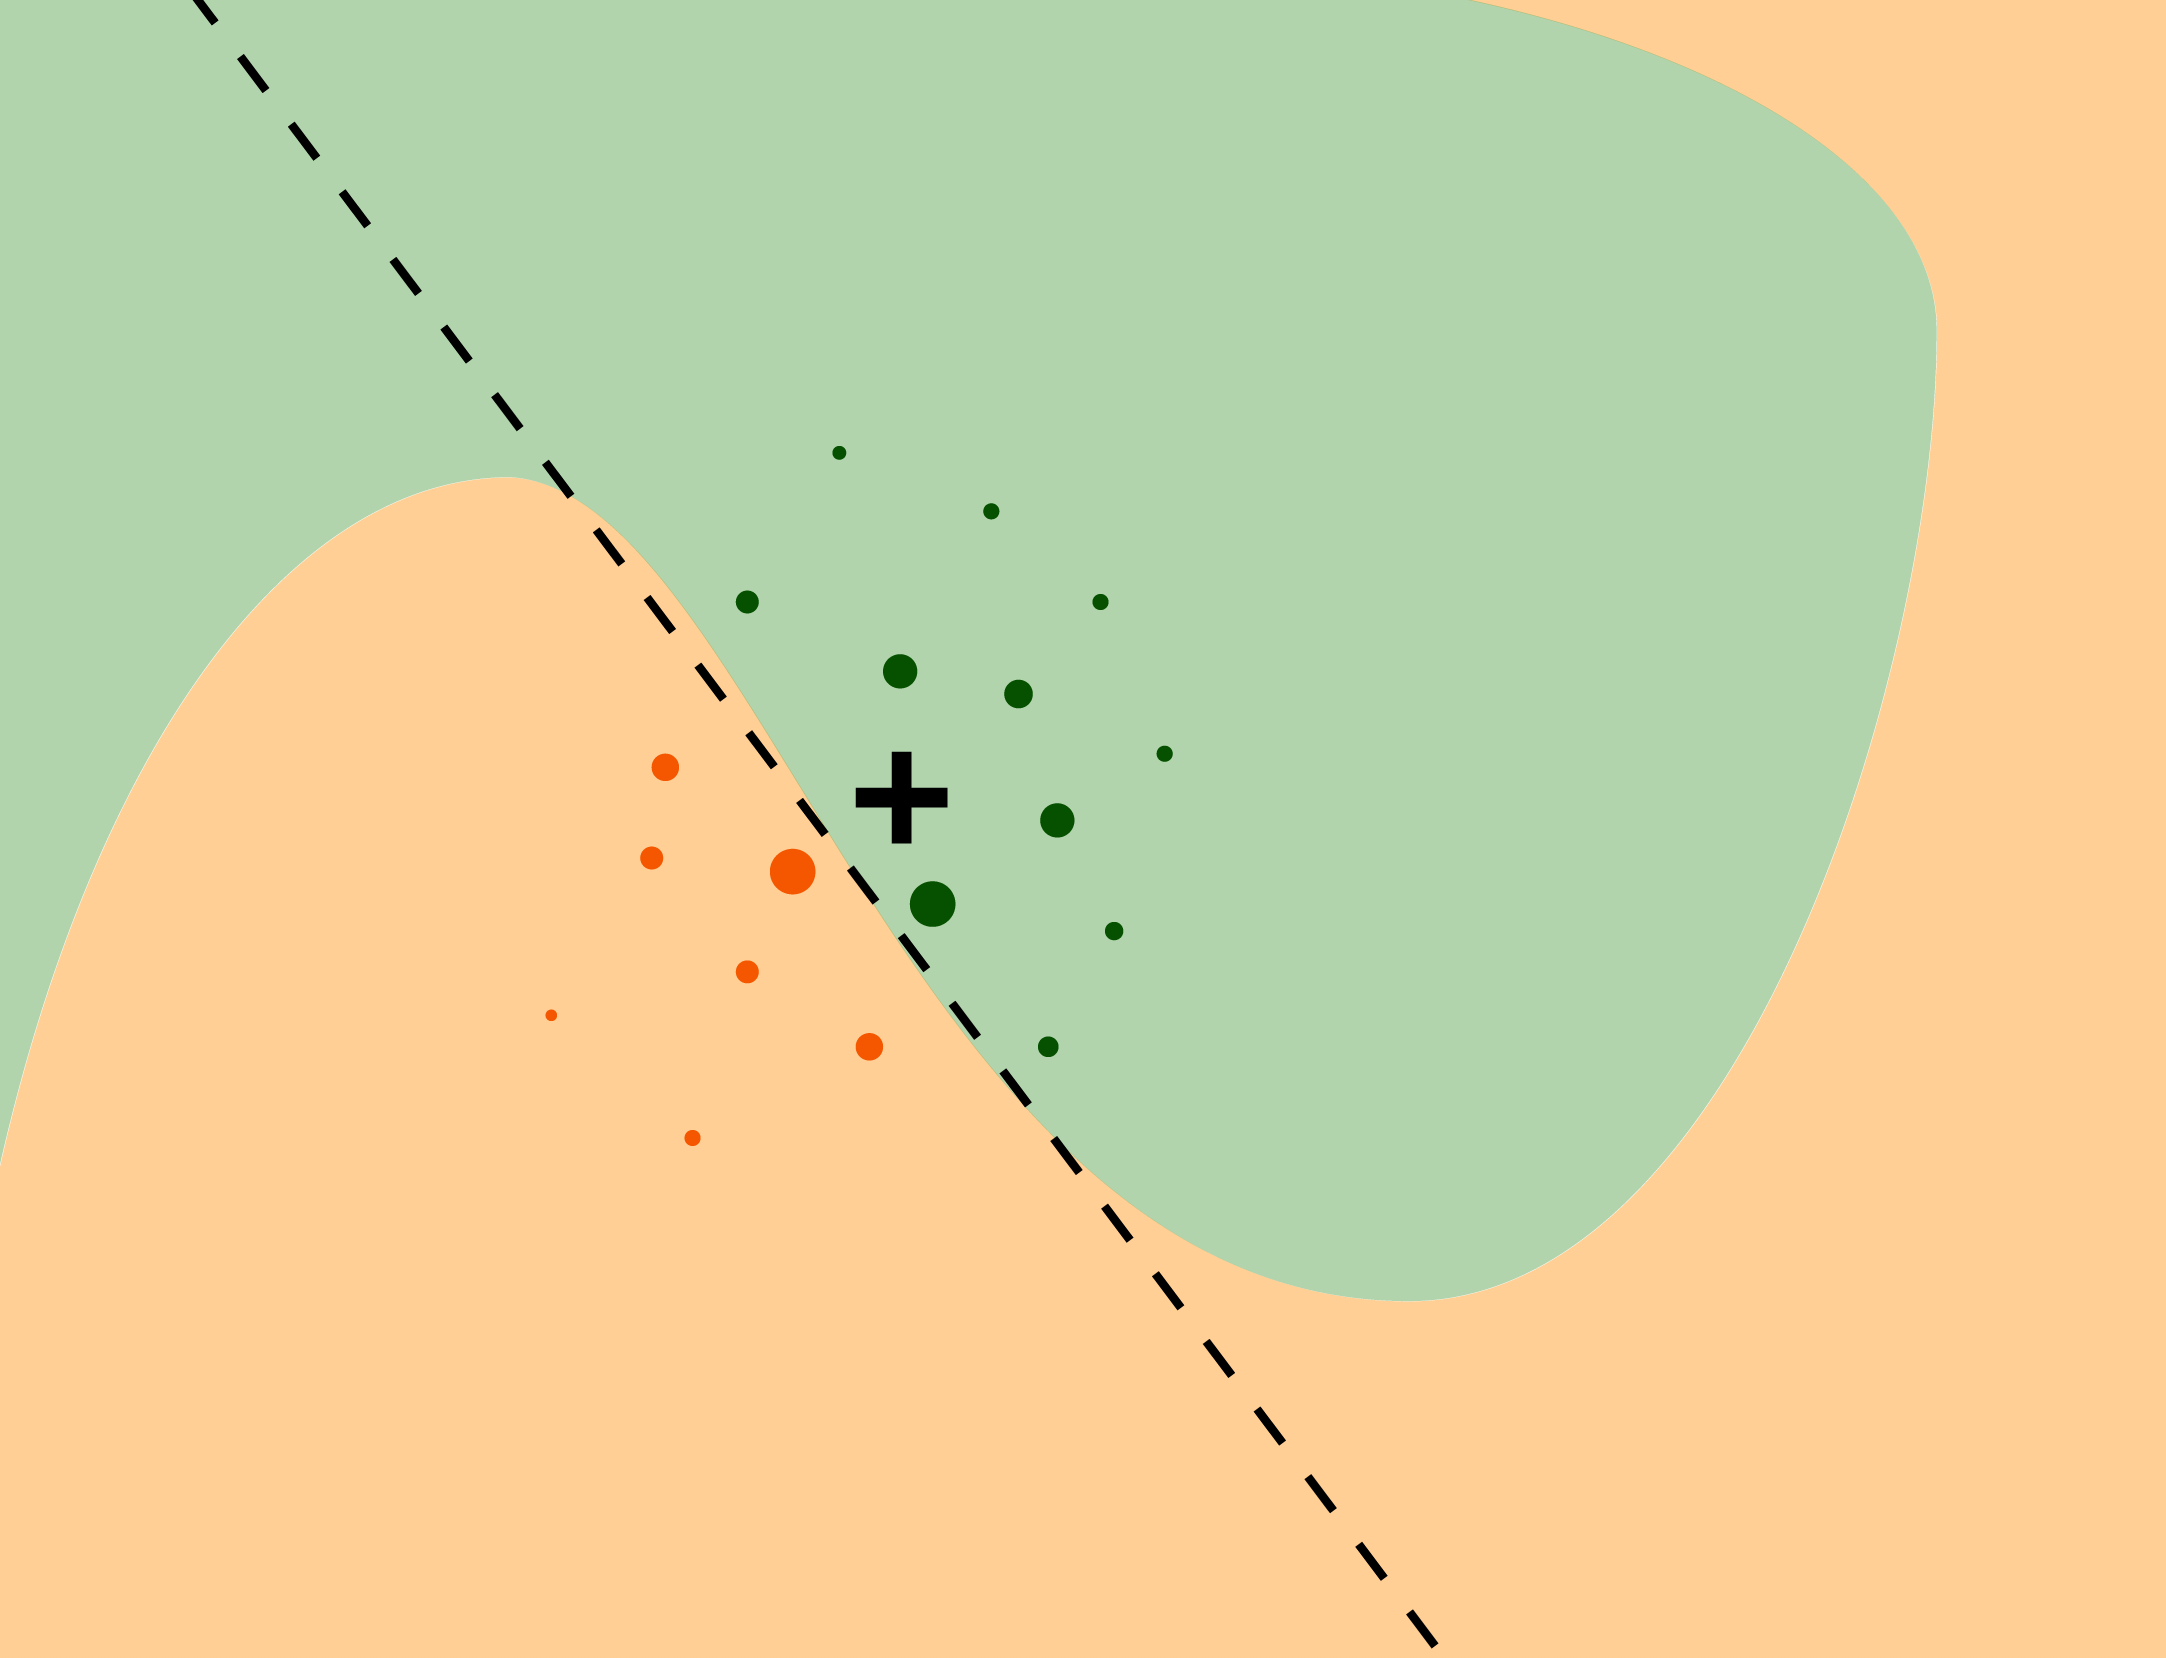
\includegraphics[width=6.5cm, height=5cm]{pics/lime4.png}
\end{minipage}

\underline{Пример LIME для табличных данных} \cite{limegit}
\vspace{-3mm}

\begin{figure}[h]
	\centering{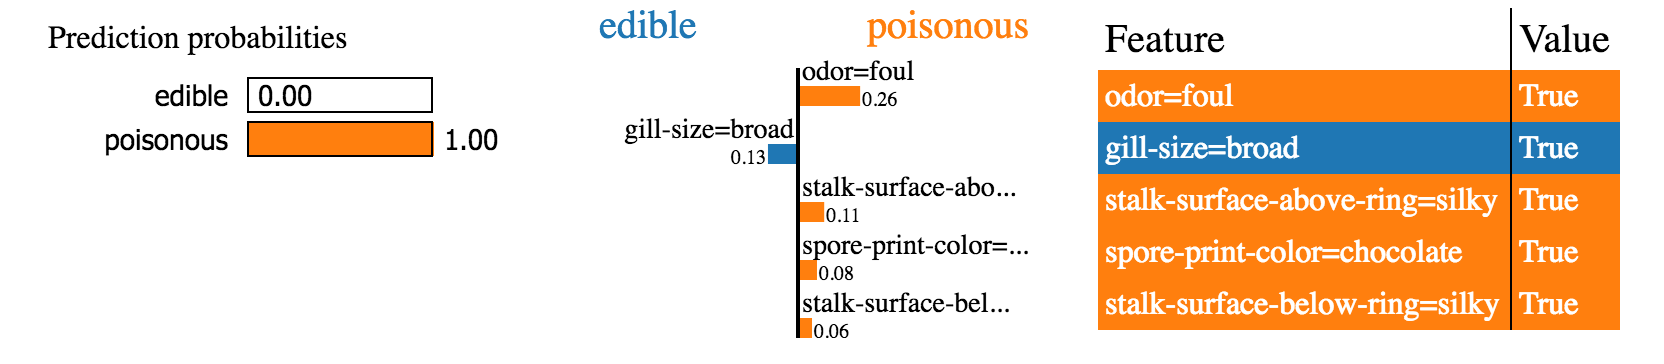
\includegraphics[width=\linewidth]{pics/lime1.png}}
\end{figure}

В данном случае решалась задача бинарной классификации. LIME вывел пять самых значимых признаков и показал, каким образом они повлияли на предсказание. Обученная модель показала, что исследуемый объект принадлежит к классу <<poisonous>>. И по анализу LIME понятно почему: только один признак из выведенных увеличил вероятность принадлежности объекта к классу <<edible>> и только на $0.13$. В то же время оставшиеся четыре признака повлияли на вероятность объекта быть <<poisonous>>, причем суммарно увеличив вероятность на $0.51$. Данная интерпретация позволяет понять, адекватна ли модель, которую мы получили, действительно ли релевантные признаки оказались значимыми.

\underline{Пример LIME для текстов} \cite{limegit}
\vspace{-3mm}

\begin{figure}[h]
	\centering{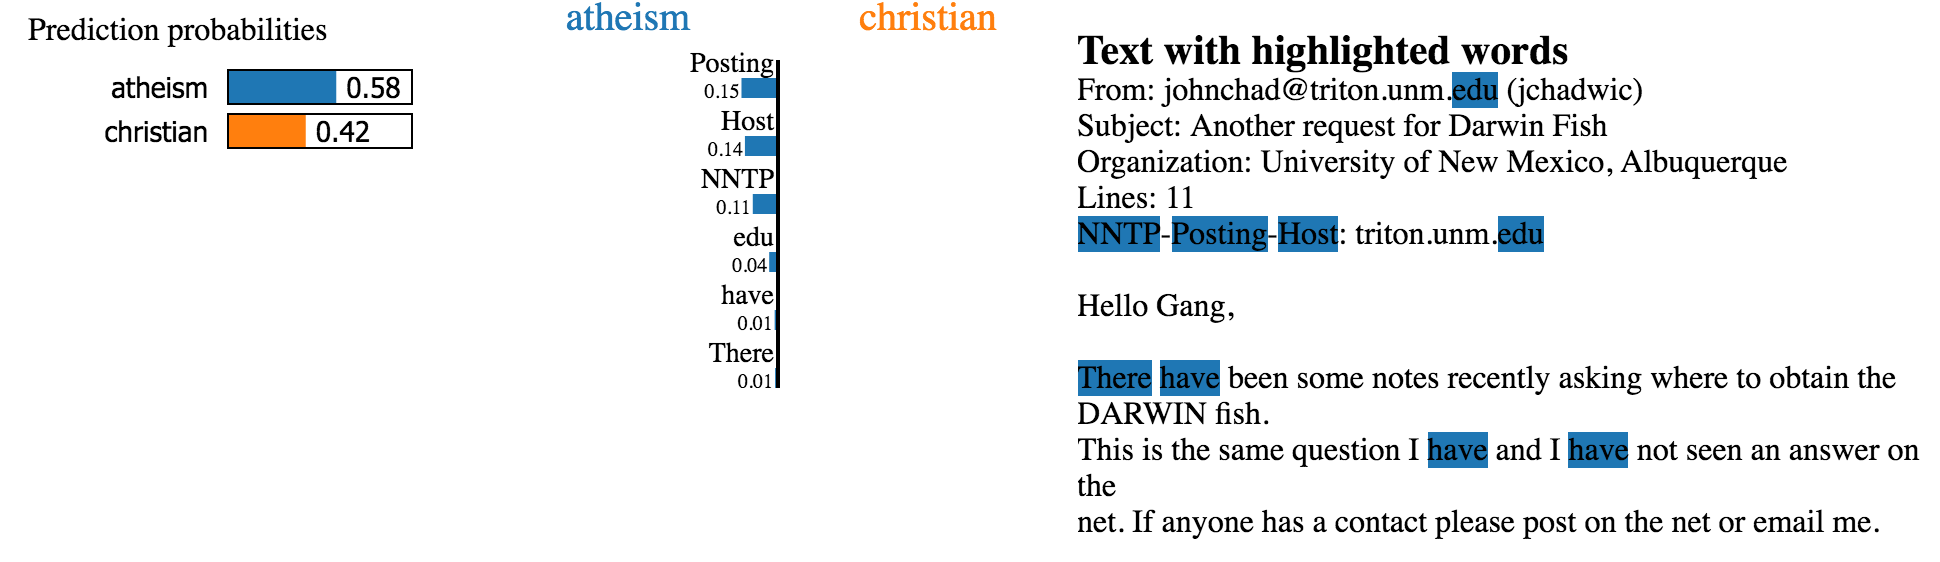
\includegraphics[width=\linewidth]{pics/lime2.png}}
\end{figure}

Вновь решалась задача бинарной классификации: определить, к какой теме (христианство/атеизм) относится документ. LIME выделил отдельные слова, которые, по его <<мнению>>, оказались наиболее важны для предсказания. Можно заметить, что слово <<Posting>> оказалось довольно-таки значимым, поскольку увеличило вероятность принадлежности текста к тематике атеизма на 0.15. Однако это несколько контринтуитивно, поскольку <<posting>> может относиться одинаково вероятно к обоим темам. Мы выявили недостаток в модели, к результатам ее работы стоит относиться аккуратно.

\underline{Пример LIME для картинок} \cite{lime_dop}
\vspace{-3mm}

\begin{figure}[h]
	\centering{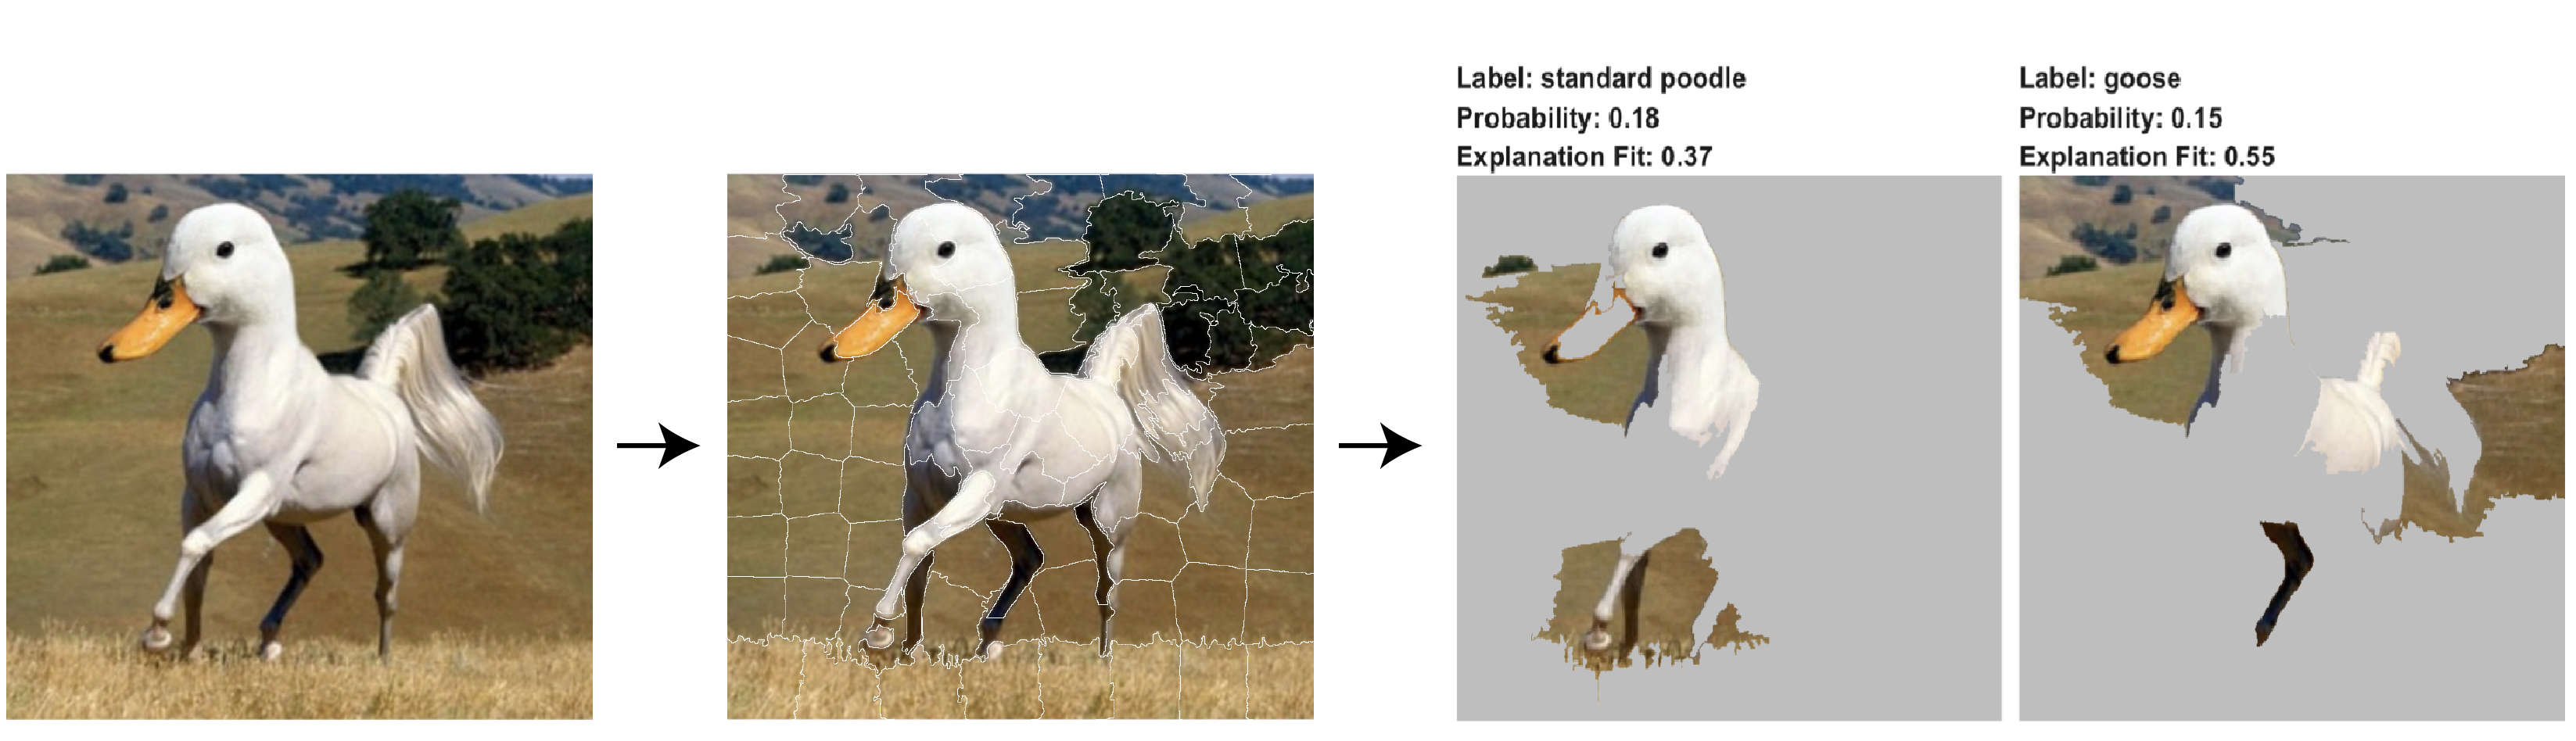
\includegraphics[width=\linewidth]{pics/lime3.png}}
\end{figure}

Интерпретация картинок с LIME наиболее понятная и интересная. Изображение было разбито на несколько частей (супер-пиксели). И далее алгоритм выбрал наиболее важные для получения того или иного ответа. Алгоритм корректно изобразил фрагменты гуся на второй картинке, которые алгоритм смог распознать. Но на первой картинке модель ошиблась и выявила пуделя.
	\subsubsection{Принцип работы}
	У нас есть модель $f(x): \re^d \rightarrow \re$ и объект $x \in \re^d$, предсказание для которого нужно интерпретировать. Мы хотим найти модель $g$ из класса интерпретируемых моделей $G$, чтобы получить из нее объяснение результата более сложной модели (например, посмотреть на веса признаков) \cite{lime}.

Сложность моделей обычно обратно зависит от ее интерпретируемости. Например, линейную модель с 2-3 предикторами гораздо проще интерпретировать, чем модель с 10 и более предикторами. Поэтому нам нужно не просто использовать более простую модель, но и преобразовать исходное пространство признаков: $x \rightarrow x'$. Нам не подходят методы снижения размерности, которые представляют признаки в уже неинтерпретируемом виде (PCA, UMAP и пр.). В данной задаче можно уменьшить количество признаков и преобразовать их \cite{lime}.

Чтобы уменьшить количество признаков, мы можем случайно выбирать некоторые из них. Либо комбинировать их между собой, при этом обращая внимание на интерпретируемость новых признаков. Для каждого типа данных подобное преобразование может проходить по-разному: для изображений -- несколько пикселей могут объединяться в один суперпиксель, для текстов -- символы объединяться в токены (например, слова -- они хорошо интерпретируются) \cite{basis}.

Для преобразования признаков существует большое количество методов. Например, приведение непрерывных переменных к дискретному виду. Основная цель подобных преобразований -- уменьшить множество значений признаков. Авторы алгоритма предлагают приводить предикторы к еще более упрощенному виду: использовать вместо признака дамми-переменную его наличия. Именно поэтому наша простая модель $g(x'):\{0,1\}^{d'} \rightarrow \re\,$ работает с интерпретируемым представлением предсказания $x' \in \{0,1\}^{d'}$, где обычно $d' << d$.
% числовые переменные можно так и оставить, они же не мешают обучаться модели. или мешают
Дополнительно в задаче вводится мера сложности $\Omega(g)$ искомой модели как регуляризация \cite{lime_dop}.

Чтобы определить окрестность рядом с $x$, внутри которой мы можем использовать простую модель, введем меру близости $\pi_x(z)$ между объектом $x$ и его соседом $z$. И наконец определим нашу функцию потерь, которую мы будем оптимизировать: $L(f, g, \pi_x)$ -- разница между моделями $f$ и $g$ в окрестности, заданной $\pi_x$. Тогда в целом задача алгоритма выглядит следующим образом \cite{lime}:
\[
explanation(x) = \xi(x) = \underset{g \in G}{\argmin} (L(f, g, \pi_x) + \Omega(g))
\]

Одной из особенностей алгоритма является его независимость от модели, которую необходимо интерпретировать. Поэтому мы не можем приписывать модели $f$ никакие свойства. Вместо этого мы будем аппроксимировать ее, искусственно создавая объекты в окрестности $x'$, переводя их в исходное пространство признаков и получая для них предсказания из $f$ \cite{lime}.

Понятие окрестности носит абстрактный характер, поэтому чтобы учесть расстояние между объектами на практике, мы будем использовать меру близости $\pi_x(z)$ как веса: чем ближе объект к $x$, тем больший вклад он вносит в функцию потерь \cite{lime}.

Гиперпараметры в задаче:\\[-8mm]
\begin{itemize}
	\item $G$ -- класс интерпретируемых моделей: линейные модели, решающие деревья и др.\\[-6mm]
	\item $d'$ -- количество признаков в новом пространстве
	\item $\pi_x(z)$ -- мера близости: например, ядра (гауссово, логистическое и др.)\\[-6mm]
	\item $D(x,z)$ -- расстояние между объектами, используемое при расчете меры близости: евклидова метрика, косинусное расстояние и др.\\[-6mm]
	\item $L$ -- функция потерь: $MSE$, $MAE$ и др.\\[-6mm]
\end{itemize}

% есть гиперпараметр К

Результат: мы получаем алгоритм, который изучает работу более сложной модели и интерпретирует ее с некоторой погрешностью -- можно изучать влияние признаков на отдельные предсказания.

	\subsubsection{Реализация}
	Данный метод реализован в библиотеке $\verb|lime|$. Она содержит в себе методы для работы с разными типами данных: $\verb|lime.lime_tabular|$, $\verb|lime.lime_text|$, $\verb|lime.lime_image|$. Инструкцию по установке можно найти \href{https://github.com/marcotcr/lime}{здесь}.
	\subsection{SHAP}
	\vspace{-1mm}
SHAP (SHapley Additive exPlanations) -- метод, оценивающий вклад признаков в предсказания модели на основе значений Шэпли.
\vspace{-3mm}

\subsubsection{Идея}
\vspace{-2mm}
Предсказание модели формируется на основе признаков. Если мы хотим узнать влияние отдельного признака, мы можем построить предсказание модели с ним и без него и затем посмотреть, как меняется результат. % почему реально не убирать насовсем?
Но модель может быть слишком сложной, чтобы мы могли оценить влияние предиктора по одному объекту, регулируя один признак при фиксированных остальных. Правильнее рассмотреть все возможные комбинации признаков: их разные значения, наличие/отсутствие, чтобы понять, как в каждом из перечисленных случаев добавление и исключение признака влияет на предсказание.

Рассматривая влияние признаков для разных объектов, мы получаем очень много предельных эффектов, что тяжело интерпретируется. Поэтому можно рассмотреть, какой в среднем эффект оказывает включение признака в модель. Тогда мы получим средневзвешенную оценку вклада отдельного предиктора в предсказание и сможем интерпретировать результат работы модели.
% Подумать, почему они сравнивают результат со средним кроме как кроме того что нужна всего одна модель и теряется точность

Однако для такого способа нужно либо обучить количество моделей, пропорциональное количеству всех комбинаций признаков -- которое растет экспоненциально с увеличением количества признаков. Либо оставлять пропущенные значения вместо исключенных признаков, что может плохо отразиться на качестве работы модели. Чтобы избежать этого, мы можем несколько видоизменить наше решение, не меняя цель. Вместо обучения дополнительной модели с меньшим количеством предикторов мы оценим ее предсказание, случайно изменяя исключенные признаки и усреднив результат.

Авторы алгоритма также вносят новую идею о способе расчета вклада признаков в предсказание: данные значения можно посчитать с помощью линейной регрессии с использованием матрицы весов определенного вида \cite{shap}.

\underline{Пример SHAP для табличных данных} \cite{shapgit}

\vspace{-4mm}
\begin{figure}[h]
	\centering{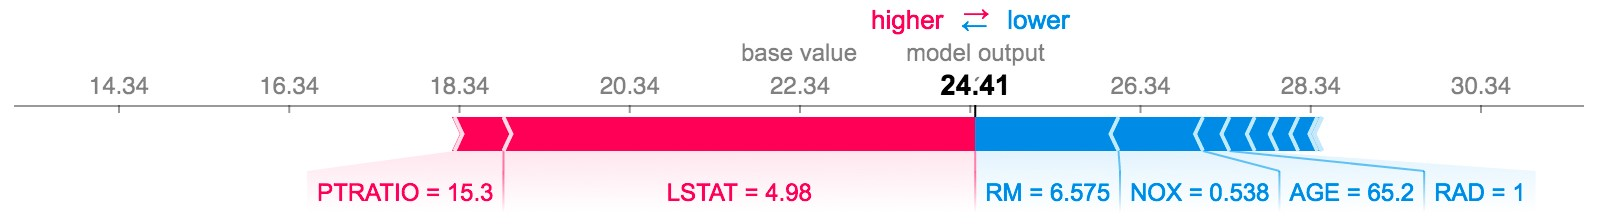
\includegraphics[width=\linewidth]{pics/shap1.png}}
\end{figure}
\vspace{-3mm}

В данном примере решалась задача регрессии, предсказание модели: 24.41. Отталкиваясь от base value как от исходного значения под воздействием влияния разных признаков (показаны стрелочками), данное наблюдение получило именно такой ответ, по мнению SHAP. Приведенные предикторы оказали наибольшее воздействие на результат работы модели. В аналогичном виде представляется интерпретация предсказаний для текстов.

\underline{Пример SHAP для картинок} \cite{shapgit}

\vspace{-2mm}
\begin{figure}[h]
	\centering{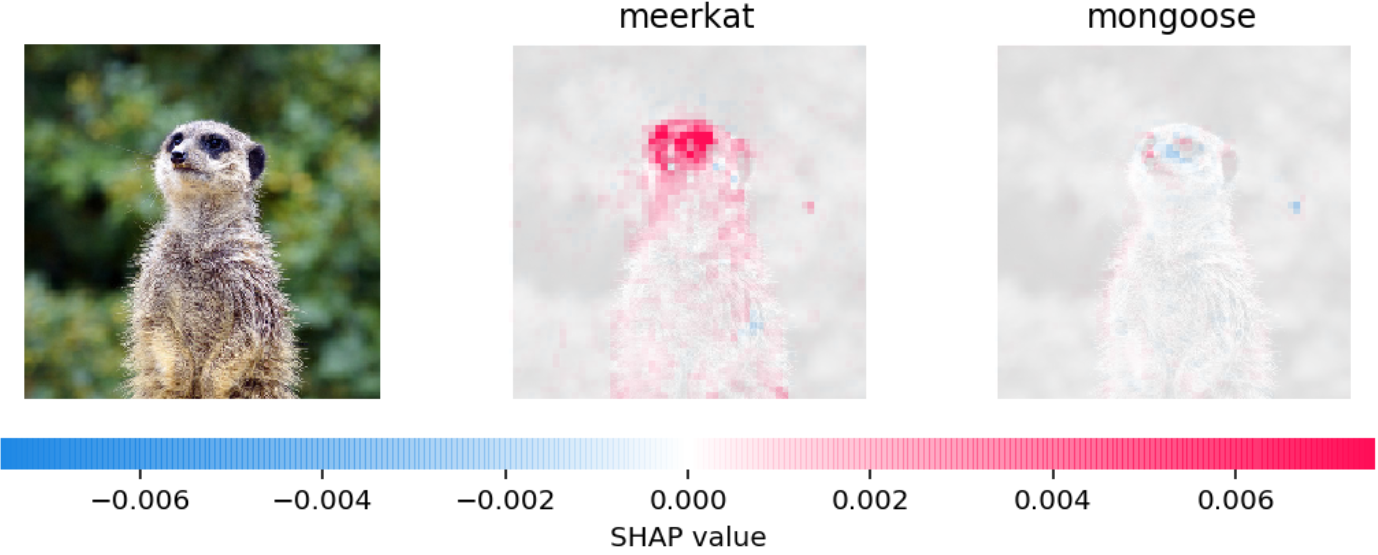
\includegraphics[width=0.65\linewidth]{pics/shap2.png}}
\end{figure}
\vspace{-2mm}

В данном случае SHAP, в отличие от LIME, работал с более мелкими признаками -- обычными пикселями. Значимость каждого признака показана с помощью цвета: чем насыщеннее цвет, тем сильнее он повлиял на результат. Красный цвет показывает положительное воздействие, синий цвет -- отрицательное. Однако SHAP может работать и с супер-пикселями, аналогично LIME.

\subsubsection{Значения Шэпли (Shapley values)}
Пусть $S$ -- множество не исключенных из модели признаков, в которое не входит исследуемый $i$-ый признак. Чтобы найти разницу предсказаний для признаков из $S$ и из $S \cup \{i\}$, куда входит $i$-ый признак, нам нужно обучить две модели, $f_S$ и $f_{S \cup \{i\}}$, соответственно. Тогда для объекта $x$ мы получим \cite{basis, shap}:
\[
f_{S \cup \{i\}}(x_{S \cup \{i\}}) - f_S(x_S),
\]
где $x_{S \cup \{i\}}$ -- объект $x$, у которого оставили только признаки из $S \cup \{i\}$, $x_S$ -- только признаки из $S$.

Как отмечалось ранее, значения данного выражения могут меняться при разных комбинациях признаков, поэтому мы усредним ее для всех возможных случаев. Считая, что $F$ -- множество всех признаков, получим итоговое выражение для $i$-го признака:
\vspace{-1mm}
\[
\phi_i = \frac{1}{|F|} \sum\limits_{S \subseteq F \backslash \{i\}}
\begin{pmatrix}
|F| - 1 \\
|S|
\end{pmatrix}^{-1}
(f_{S \cup \{i\}}(x_{S \cup \{i\}}) - f_S(x_S)),
\]
\vspace{-5mm}

где $|F|$ -- количество элементов в множестве $F$, $|S|$ -- в множестве $S$ \cite{basis, shap}.

Коэффициент:
\[
\ds \begin{pmatrix}
|F| - 1 \\
|S|
\end{pmatrix} = \frac{(|F|-1)!}{|S|! \cdot (|F| - |S| - 1)!}
\]
равен количеству всех возможных комбинаций признаков без учета исследуемого. Поделив на него, а также на количество признаков получаем среднее значение вклада признака.

Данный коэффициент также можно интерпретировать как вес комбинации при расчете среднего. Биномиальный коэффициент, равный количеству комбинаций, для одного или $|F|-1$ признаков меньше, чем для любого другого числа признаков. При делении на коэффициент мы получаем большее значение, который указывает на больший вес подобных комбинаций. Это имеет смысл, так как больше информации мы получаем, рассматривая влияние признаков по отдельности: либо оставляя только его, либо исключая все кроме него. С увеличением количества признаков в $S$ вес комбинации убывает.

Таким образом, мы получили величину, показывающую, какой в среднем вклад вносит конкретный признак в предсказание. Данное значение пришло из теории игр и носит название значение Шэпли (Shapley value). Они показывают, какой вклад внес в общий выигрыш отдельный игрок при кооперации. В нашей задаче мы рассматриваем предсказание модели как выигрыш, а признаки как игроков \cite{basis}.
\vspace{-2mm}
	\subsubsection{Принцип работы}
	Метод SHAP несколько отличается от использования значений Шэпли напрямую для интерпретации вклада признаков -- он модифицирует классический подход. Рассмотрим SHAP подробнее.

Вместо использования большого количества моделей мы обучим одну модель и далее будем пользоваться только ее предсказаниями. Тогда наша модель представима в виде $f: \re^d \rightarrow \re$. Вместо исключения из нее признаков (в таком случае нам пришлось бы переобучать модель) мы оставим данные признаки в виде случайных величин и посчитаем математическое ожидание предсказания при фиксированных включенных в модель признаках \cite{basis, shap}.

Для упрощения расчетов мы не будем рассматривать разные значения предикторов, а бинаризуем их представление, обозначив за <<1>> наличие предиктора и за <<0>> его отсутствие: $x \rightarrow x', \, x' = \{1\}^d$. % не знаю корректно ли
Обозначим за $z' \in \{0,1\}^d$ объект, у которого мы учитываем только признаки из $S$ при формировании предсказания:
$z_j =
\begin{cases}
1, \text{если $j \in S$}\\
0, \text{если $j \notin S$}\\
\end{cases}$.\\
То есть $z'$ -- одна из возможных комбинаций предикторов \cite{basis, shap}.

Обученная модель работает с исходным видом признаков, поэтому нам нужно также восстанавливать значения исходных признаков по бинарному вектору. Введем для этого функцию $h_x(z') = z$, где $x$ -- исходный вектор исследуемого объекта, $z'$ -- бинарный вектор, в котором некоторые признаки заменены нулями, $z$ -- представление вектора $z'$ в исходном пространстве признаков \cite{basis}.

\vspace{-3mm}
\begin{figure}[h]
	\centering{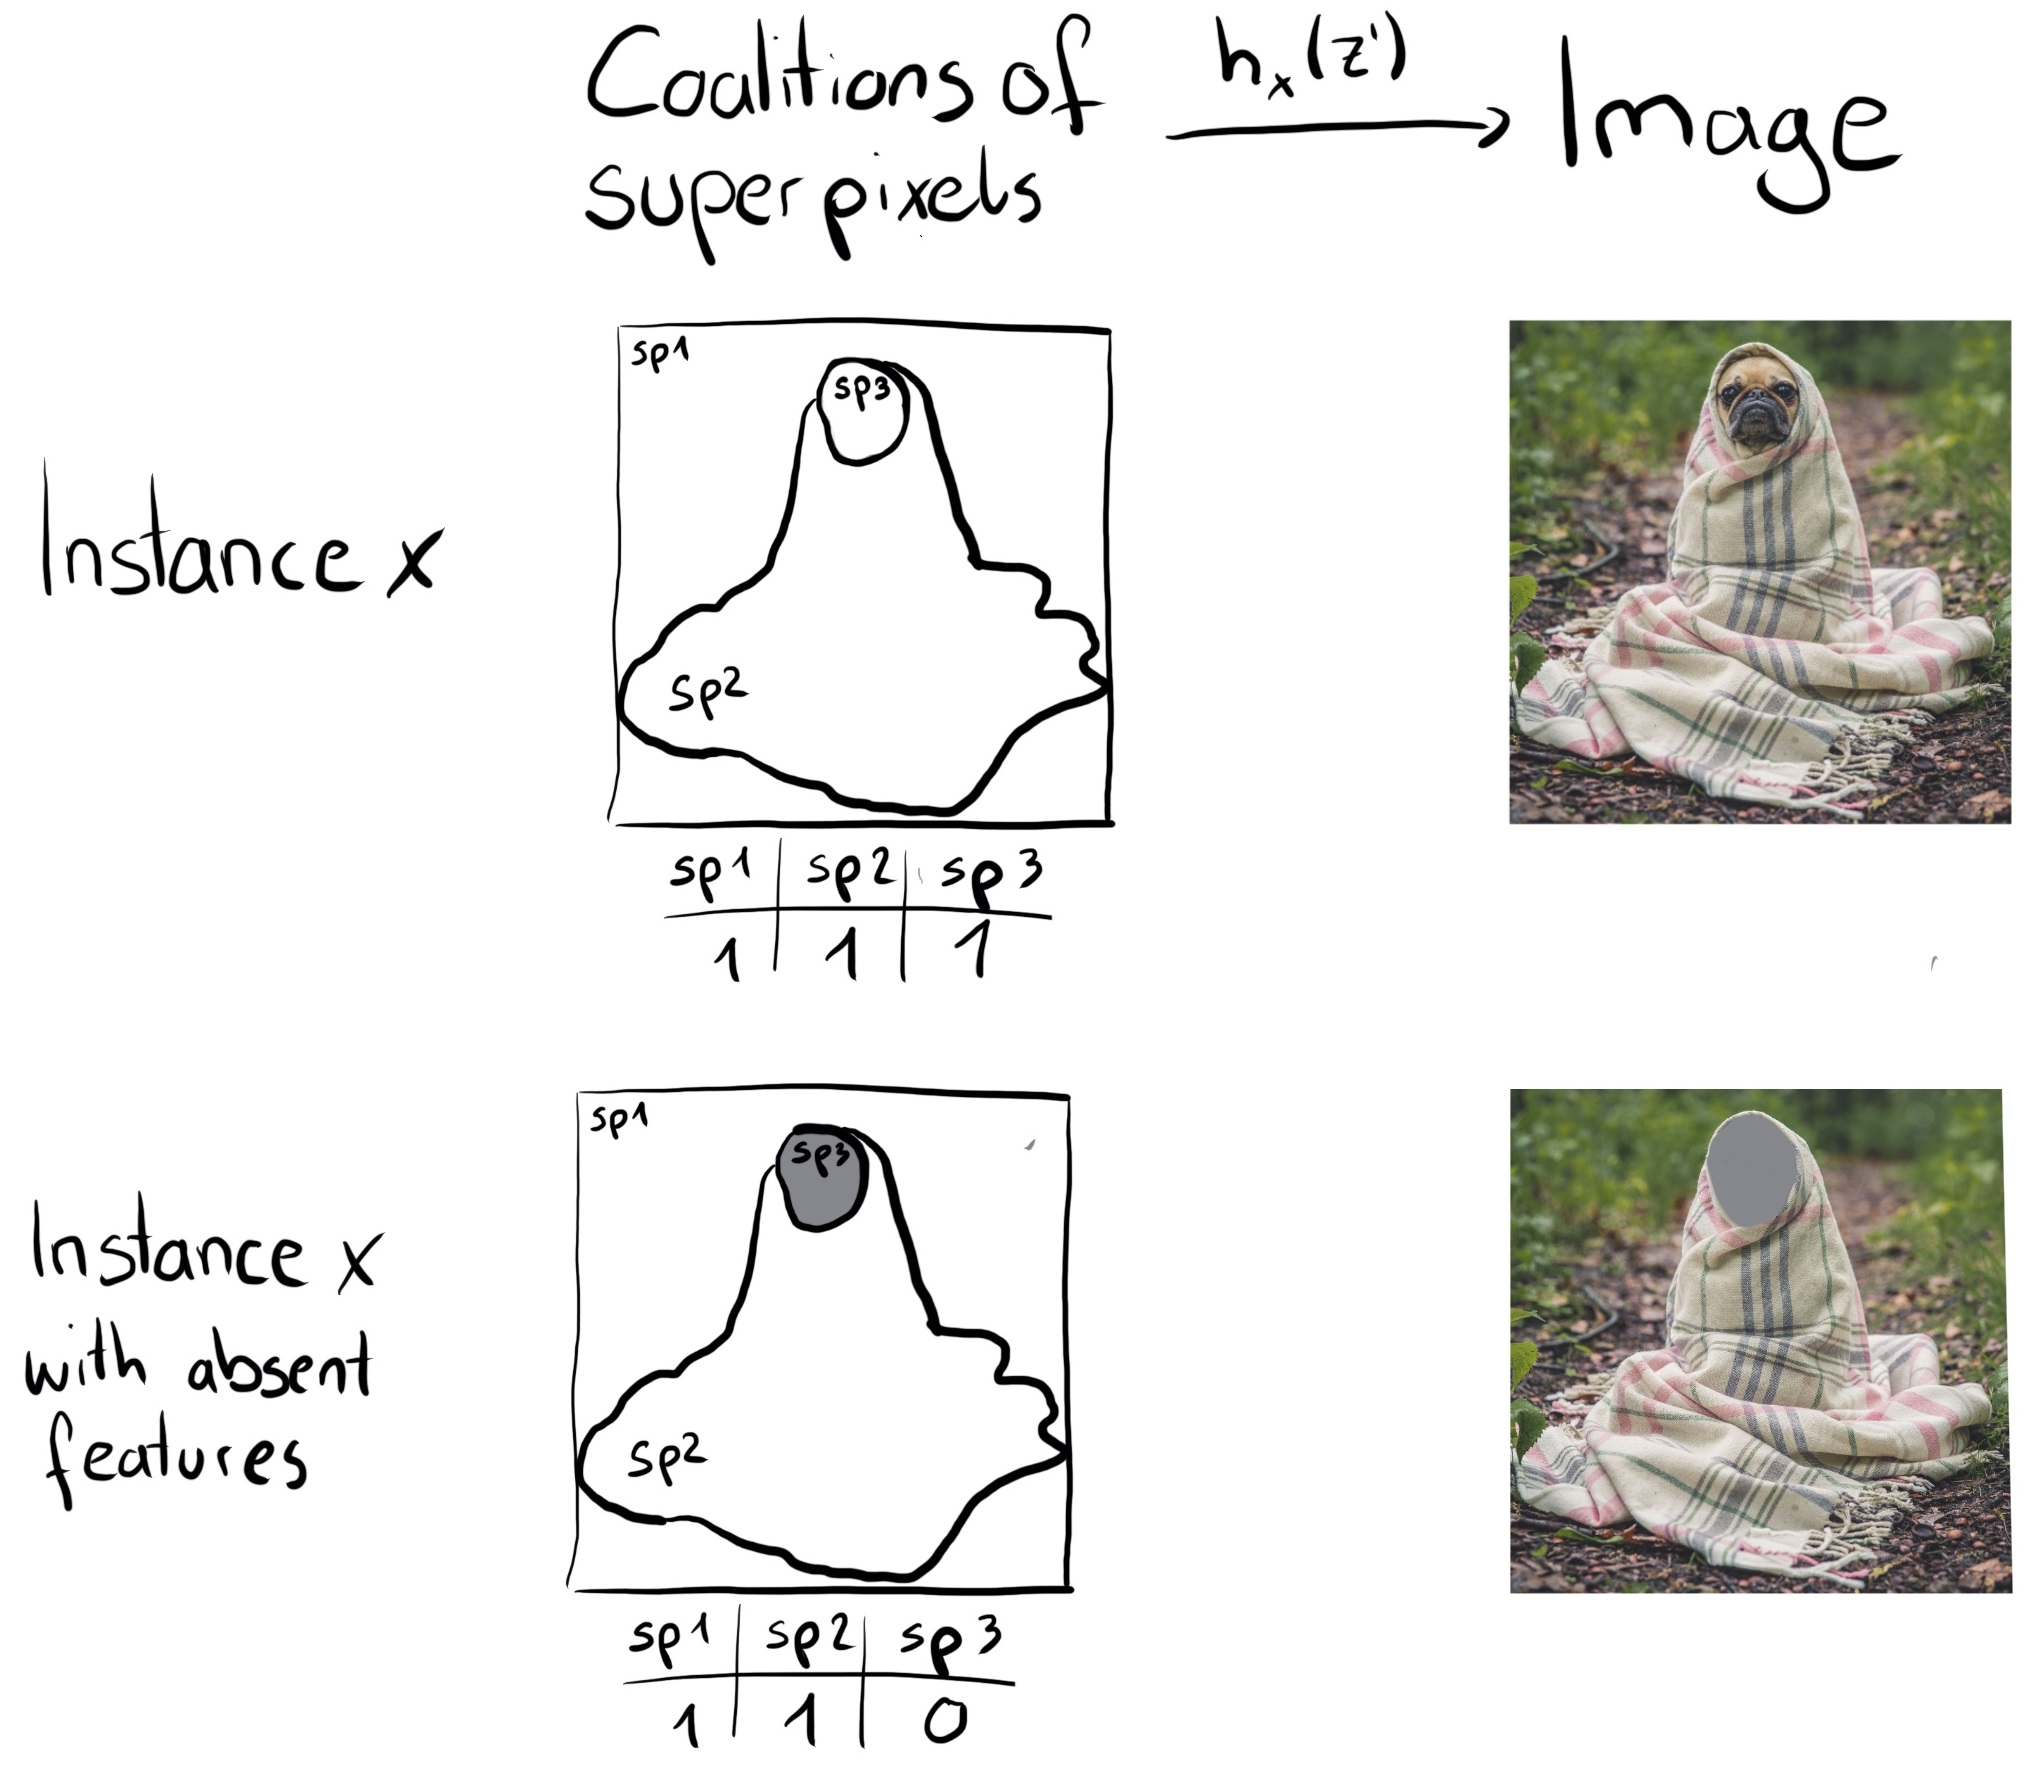
\includegraphics[width=0.6\linewidth]{pics/shap3.png}}
\end{figure}
\vspace{-3mm}

Функция $h_x$ вместо единиц восстанавливает значения из вектора $x$, а вместо нулей оставляет признак как некоторую переменную (случайную величину).
% наверняка можно как-то умнее упрощать признаки
Тогда наше ожидаемое предсказание для $z$ представимо в виде математического ожидания:
\[
\bar{f}(z) = \e(f(z)|\,z_S)
\]

Мы знаем конкретные значения признаков $z_S$, так как функция $h_x$ перенесла их из объекта $x$. Найдя математическое ожидание мы можем подставить данные значения, чтобы получить условное математическое ожидание, которое и будет оценкой нашего предсказания. Данную формулу мы можем использовать при расчете необходимых значений \cite{basis}.% здесь для его расчета мы почему-то переходили к безусловному матожиданию, это связано со свойствами значений Шэпли -- не уверена нужно ли это прописывать

Поскольку мы не знаем истинное распределение, чтобы иметь возможность посчитать матожидание, аппроксимируем его оценкой. Для этого немного изменим функцию $h_x$ -- теперь вместо нулей она будет проставлять случайные значения соответствующих признаков. Тогда для каждого множества $S$ мы сможем получить несколько предсказаний модели и усреднить их \cite{basis}:
\[
\hat{f}(z) = \frac{1}{k} \sum\limits_{i=1}^k f(z_{F\backslash S}, z_S),
\]
где $z_{F\backslash S}$ -- исключенные из модели признаки, вместо которые подставлены случайные значения, $z_S$ -- включенные в модель признаки, значения которых известны из исследуемого объекта $x$.
\vspace{-2mm}

\paragraph{Kernel SHAP.}% я очень хочу доказать то, что они доказали
Авторы алгоритма показали, что есть упрощенный способ найти значения Шэпли: % с оговоркой про то что это не значения Шэпли
с помощью взвешенного МНК. В нем аналогично перебираются разные комбинации $z'$ -- так формируется выборка $Z$ для регрессии. Зависимой переменной является предсказание модели для сгенерированной выборки (переведенной в исходное пространство признкаов): $y_i = f(h_x(z'_i)) = f(z_i)$, где $z'_i$ -- строка матрицы $Z$. Тогда решением нашей задачи является вектор \cite{basis}: \[
\phi = (Z^T W Z)^{-1} Z^T W y
\]
\vspace{-6mm}
% нужно ли говорить про корреляцию признаков. они это указывают как раз при расчете условного матожидания, и здесь наверное аналогия в мультиколлинеарности, но это неточно

Чтобы коэффициенты в регрессии соответствовали искомым значения, веса должны быть заданы диагональной матрицей $W$ \cite{shap}: 
\[w_{ii}(z'_i) = \frac{|F|-1}{
	\begin{pmatrix}
	|F| \\
	|S_i|
	\end{pmatrix} \cdot |S_i| \cdot (|F| - |S_i|)} = \frac{|F|-1}{|F|} \cdot \frac{|S_i - 1|! \cdot (|F|-|S_i|-1)!}{(|F|-1)!},
\]
где $|S_i|$ -- количество элементов в множестве $S_i$, то есть количество ненулевых элементов в $z'_i$.

В данном случае коэффициент при константе будет показывать предсказание модели при отсутствии признаков. Коэффициенты при признаках являются соответствующими значениями Шэпли, % если так можно сказать. мб сноска
которые можно использовать для интерпретации их вклада в предсказание \cite{basis}.

Ранее мы уже говорили о том, что комбинации, в которых либо почти все нули, либо почти все единицы имеют больший вес при расчете значений Шэпли. Данный факт сохраняется и в линейной регрессии, поэтому формируя выборку можно отдавать предпочтение именно данным примерам -- в случае, если мы ограничены в количестве наблюдений \cite{basis}.

Интересно, что если записать задачу в более общем виде:
\[
\sum\limits_{z' \in Z} (f(h_x(z')) - g(z'))^2 \cdot \underbrace{\frac{|F|-1}{|F|} \cdot \frac{|S - 1|! \cdot (|F|-|S|-1)!}{(|F|-1)!}}_{w(z') = \pi_x(z')} = L(f, g, \pi_x) + \Omega(g) \rightarrow \min_g
\]
\vspace{-4mm}

мы получим ровно ту же задачу, что решает LIME. То есть при определенных гиперпараметрах LIME и SHAP эквивалентны друг другу \cite{shap}.
% регуляризация -- легально ли это, мы ведь хотим значения Шэпли хммм
% сказать что бесконечные веса -- я как-то устранила :О

Существуют и другие модификации SHAP: TreeSHAP, Linear SHAP, Low-Order SHAP, Max SHAP, Deep SHAP и др. В отличие от классического подхода они специфицированы для отдельных классов моделей, что позволяет снизить время работы алгоритма \cite{basis, shap}.
	\subsubsection{Реализация}
	Данный метод реализован в библиотеке $\verb|shap|$. Универсальный метод содержится в модуле: $\verb|shap.KernelExplainer|$. Модицикации перечисленные ранее являются более специлизированными:\\[-8mm]
\begin{itemize}
	\item $\verb|shap.TreeExplainer|$: XGBoost/LightGBM/CatBoost/scikit-learn/pyspark models\\[-7mm]
	\item $\verb|shap.DeepExplainer|$: TensorFlow/Keras models\\[-7mm]
	\item $\verb|shap.GradientExplainer|$: TensorFlow/Keras/PyTorch models\\[-7mm]
	\item и др.
\end{itemize}.
\vspace{-7mm}

Инструкцию по установке можно найти \href{https://github.com/slundberg/shap}{здесь}.
	\newpage

	\section{Анализ данных и интерпретация}
	Рассмотрим описанные методы на конкретной задаче. Построим относительно сложную модель (градиентный бустинг) для бинарной классификации объектов.
	\subsection{Данные}
	Для анализа был выбран датасет, содержащий информацию о клиентах разных отелей за 2015-2017 года. Описание датасета можно найти в \href{https://www.kaggle.com/jessemostipak/hotel-booking-demand}{здесь}. Задача: предсказать, отменит ли клиент бронь. Датасет был предварительно обработан:
\begin{itemize}
	\item Удалены переменные company (много пропусков), agent (ID туристических агенств -- зависит от приведенной классификации), reservation status, reservation status date (данная информация обычно бывает известна уже после отмены либо отъезда гостя), arrival date year, arrival date month (данные представлены только по 2015-2017 годам, слишком мало информации для предсказаний на более дальние периоды; месяц аналогично несет мало информации -- вместо данных переменных осталась переменная arrival date week number)
	\item Стандартизированы все числовые переменные, кроме arrival date week number, arrival date day of month (порядковые переменные), is repeated guest (бинарная переменная)
	\item Приведены к числовому виду порядковые переменные meal, deposit type, reserved room type, assigned room type
	\item Приведены к бинарному виду категориальные переменные hotel, country, market segment, distribution channel, customer type
	\item Удалены строки с пропущенными значениями -- таких строк было немного и в них была пропущена важная информация
	\item Удален выброс: для одного наблюдения adr $<0$, что не может быть правдой, так как adr $> 0$
\end{itemize}
	\subsection{Модель}
	Для анализа описанных методов я выбрала модель бинарной классификации XGBoost. Подбор гиперпараметров осуществлялся с помощью кросс-валидации на тренировочных данных. Одной из проблем данных является их несбалансированность: она решалась учетом объектов положительного класса с большим весом. Посмотреть на процесс кросс-валидации и обучения модели можно \href{https://github.com/elizacc/CW/blob/master/data%20%26%20code/XGBoost_%26_analysis.ipynb}{здесь}
	\newpage
	\subsection{Интерпретация результатов}
	Модель достигла неплохого качества в задаче классификации: ROC-AUC=0.905, accuracy=0.824. Попробуем интерпретировать ее результаты.

\textbf{Нулевой способ это встроенный метод XGBoost}, показывающий важность признаков при предсказании. Посмотрим на первые 5 самых важных признаков. Данная величина может быть расчитана тремя способами: <<weight>>, <<gain>>, <<cover>>. Первый показывает, сколько раз признак появляется в дереве:

\begin{figure}[h]
	\centering{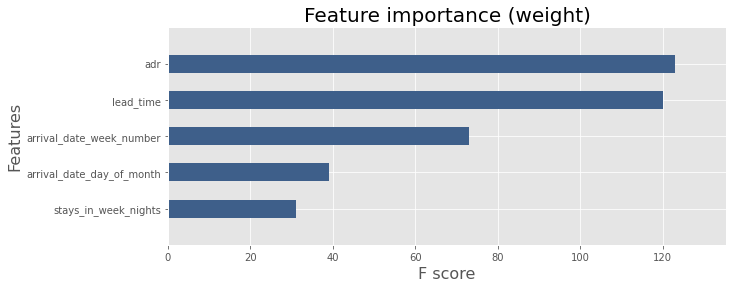
\includegraphics[width=0.85\linewidth]{pics/imp1.png}}
\end{figure}

Второй -- на сколько в среднем уменьшалась ошибка при использовании данного признака:

\begin{figure}[h]
	\centering{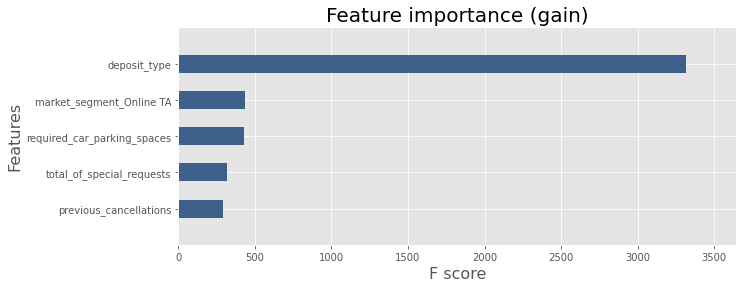
\includegraphics[width=0.85\linewidth]{pics/imp2.png}}
\end{figure}

И последний -- какое количество объектов выборки задействовало узлы с заданным признаком:

\begin{figure}[h]
	\centering{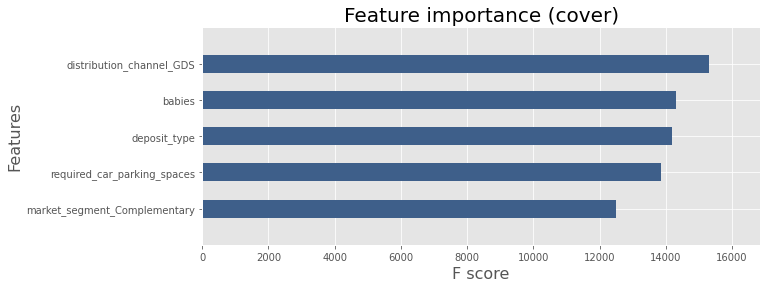
\includegraphics[width=0.85\linewidth]{pics/imp3.png}}
\end{figure}

Теперь перейдем к описанным ранее методам. \textbf{Первый -- PDP}. Возьмем признаки, которые сам XGBoost посчитал наиболее важными: первые два из weight (adr, lead\_time), первый из gain (deposit\_type) и первый из cover (distribution\_channel\_GDS) -- они с отрывом выходят в лидеры.

И также возьмем признаки, которые XGBoost счел самыми незначительными: последний из weight (distribution\_channel\_GDS, забавно -- в тренировочной выборке всего 145 объектов, которым соответствует GDS. Судя по всему данный признак встречается 1-2 раза в узлах деревьев, но при этом он отсекает очень много объектов, из-за чего cover считает его важным), последний из gain (customer\_type\_group) и последний из cover (market\_segment\_Offline TA/TO).

Построим для них PDP.

\begin{tabular}{c|c}
	\arrayrulecolor[rgb]{0.8,0.85,1}
	\includegraphics*[width = 0.47\textwidth]{pics/mypdp1.png} & \includegraphics*[width = 0.47\textwidth]{pics/mypdp2.png}\\
	\hline
	\includegraphics*[width = 0.47\textwidth]{pics/mypdp3.png} & \includegraphics*[width = 0.47\textwidth]{pics/mypdp4.png}\\
	\hline
	\includegraphics*[width = 0.47\textwidth]{pics/mypdp5.png} & \includegraphics*[width = 0.47\textwidth]{pics/mypdp6.png}\\
\end{tabular}\\[2mm]

Первый признак является непрерывным, второй --  дискретным, третий -- порядковым, остальные -- бинарными. Для первых двух видно распределение значений признака (штриховка под графиком) и коридор, показывающий как данный признак влиял на разные объекты в выборке. Для остальных: выборка была кластеризована, и для каждого кластера из 1000 была построена усредненная по подвыборке кривая.

По графикам видно, что:
\begin{itemize}
	\item признак adr оказался важным с точки зрения PDP -- для больших значений (> 50) он вносит положительный вклад в прогноз, увеличивая вероятность отмены брони. Но видно, что для некоторых объектов в выборке он оказывал также и отрицательное влияние -- коридор задевает область отрицательных значений.
	
	Данный признак показывает, сколько в среднем гость тратит на проживание и связанные с ним расходы. Исходя из графика, можно сделать вывод, что чем больше предстоящие расходы, тем выше вероятность отмены брони -- звучит логично, клиент вероятнее отменит бронь, если для него эта поездка окажется слишком дорогой. Причем вклад данного признака стабилизируется с ростом затрат и составляет +0.2 к вероятности отмены в среднем
	
	\item Аналогичный график у lead time (время от открытия брони до приезда).
	
	Здесь ситуация также интуитивно понятна: если гость очень заранее забронировал номер, то за время до приезда его планы могут поменяться. Поэтому клиент вероятнее отменит бронь в данном случае -- +0.2-0.4 к вероятности отмены
	
	\item deposit type также оказался важным признаком: в среднем он оказывает положительное воздействие на предсказание, которое доходит вплоть до полного влияния в виде +0.9 к вероятности. Ни для одного кластера признак не оказывает отрицательное воздействие, однако возможно для отдельных объектов это неверно -- важно аккуратно интерпретировать результаты.
	
	Здесь результат несколько контринтуитивен. Если у клиента есть полный предоплаченный депозит, который не возвращается, то вероятность отмены брони стремится к единице, что нелогично -- внесенный залог должен мотивировать гостей приезжать. Далее мы видим, что для большинства кластеров при переходе к возвращаемому частичному депозиту вероятность практически не меняется и остается около единицы -- это уже более логично, однако также спорно: в случае отмены придется тратить время на бюрократию, связанную с возвратом средств. Но для части кластеров при переходе к возвращаемому депозиту вероятность отмены даже падает, что вызывает сомнения в корректности использования данного признака. Возможно, стоило выбрать другую форму для данного признака: сделать его бинарным, а не порядковым -- то есть, возможно, данная ситуация сложилась из-за неправильного представления категорий депозита.
	
	\item distribution channel GDS отрицательно влияет на предсказание, причем довольно-таки сильно: при переходе от 0 к 1 вероятность отмены брони снижается в среднем на 0.1, максимально по кластерам на 0.3
	
	Данный признак показывает то, что гость воспользовался глобальной системой бронирования, то есть вероятно самостоятельно организовал себе поездку. Снижение вероятности в данном случае не очень логично: человеку проще отменить поездку, когда он ее организовал сам. Также в таком случае выше шанс возникновения проблем в поездке (по сравнению с ораганизацией, предоставляемой туристическими агентствами), из-за чего бронь также может быть отменена
	
	\item у customer type group похожий график, однако влияние существенно ниже. Вероятность снижается на 0.04 в среднем, максимально по кластерам всего лишь на 0.1
	
	График показывает, что при организации групповой поездки ниже шанс, что она отменится. Исходно не очень понятно: если бронь на группу, то она вероятнее отменится, потому что сложно организовать путешествие на целую группу, или она вероятнее не отменится из-за, например, обязательства каждого перед другими (чтобы не ставить людей из своей группы в неудобное положение). То есть данный график приносит некоторое дополнение к нашим данным. Теперь мы знаем, что если поездка организуется для группы, то бронь скорее не будет отменена -- учитываем данное дополнение с осторожностью, учитывая неточность метода
	
	\item признак market segment offline TA/TO оказался незначительным, в среднем он вносит нулевой вклад в предсказание. Однако по кластерам видно, что разброс существенный. То есть данный признак оказывает влияние на каждый отдельный объект -- PDP в виде усредненной кривой не совсем корректный выбор для интерпретации в данном случае, так как он не учитывает разброс
\end{itemize}

Построим также графики взаимодействия признаков (PDP для двух признаков)\footnote{При построении второго типа графика (contour), который показывает линии уровня может возникнуть ошибка. Это связано с несоответствием версии библиотеки matplotlib}. Посмотрим на совместное влияние признаков, которые XGBoost по критерию weight счел важными: adr и lead time.

\begin{tabular}{c|c}
	\arrayrulecolor[rgb]{0.8,0.85,1}
	\includegraphics*[width = 0.5\textwidth]{pics/mypdp7.png} & \includegraphics*[width = 0.42\textwidth]{pics/mypdp8.png}\\
\end{tabular}\\[2mm]

Данный график показывает не влияние предикторов, а непосредственно предсказание. Действительно, взаимодействие данных признаков меняет картину (то есть предсказание не линейно зависит от них). Разброс значений наблюдается с 0.199 до 0.772, разница в 0.573. Особо выделяется пик, который сложился именно из взаимодействия -- желтый островок со значениями 0.7+

В целом мы видим, что при росте времени до приезда и затрат вероятность растет. И выделяется особый случай, когда затраты не очень большие, а время до приезда велико -- в таком случае вероятность отмены брони максимальна.
\newpage
Также интересно узнать, станет ли market segment offline TA/TO более значимым в сочетании с другим, например, с lead time.

\begin{tabular}{c|c}
	\arrayrulecolor[rgb]{0.8,0.85,1}
	\includegraphics*[width = 0.44\textwidth]{pics/mypdp9.png} & \includegraphics*[width = 0.44\textwidth]{pics/mypdp10.png}\\
\end{tabular}\\[1mm]

Рассмотрение двух признаков привело к появлению влияния market segment offline TA/TO -- при больших значениях lead time он становится более значимым, его предельный эффект при lead time $=709$ в среднем составляет $0.572-0.633=-0.06$, что по модулю больше нуля. При малых значениях lead time он перестает влиять на предсказание. Это отличается от результатов, полученных ранее.

Получили добавку к интерпретации market segment offline TA/TO -- если поездка организована туроператором, то она менее вероятно отменится, что интуитивно понятно.

С помощью PDP мы убедились в корректности восприятия моделью некоторых признаков. Для других -- в контринтуитивности результатов, а также нашли возможность для пересмотра формата признаков с целью улучшения модели. Стоит отметить, что в PDP есть очевидный недостаток -- если признак равен 0, то его влияние также равно 0, что не всегда правда. Важно обращать на это внимание при интерпретации.

\textbf{Перейдем к следующему методу -- LIME}. Рассмотрим конкретную поездку (первая из тренировочной выборки), чтобы увидеть, какие признаки оказались наиболее важными для предсказания отмены брони. Истинное значение для данного объекта: 0, то есть бронь не была отменена. 

\vspace{-2mm}
\begin{figure}[h]
	\centering{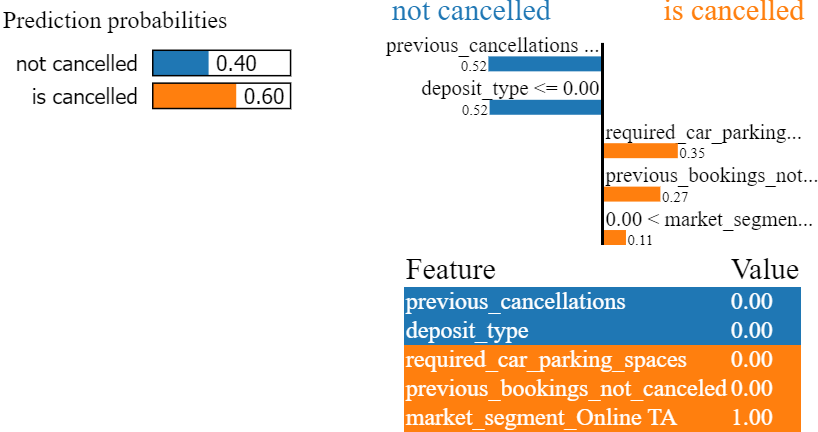
\includegraphics[width=0.7\linewidth]{pics/mylime1.png}}
\end{figure}
\vspace{-2mm}

Модель предсказала, что бронь будет отменена, и LIME с некоторой погрешностью показывает нам, что на это повлияло. Мы видим, что отсутствие отмен ранее снизило вероятность текущей отмены, что корректно. Снова столкнулись с признаком deposit type -- отсутствие депозита также снизило вероятность отмены -- в целом не противоречит ничему, однако отсутствие депозита позволяет без каких-либо потерь отменить бронь, то есть все же скорее увеличивает вероятность отмены с точки зрения интуиции. Два данных признака сильнее всего повлияли на снижение вероятности отмены: -0.52 от каждого.

Клиент не запросил парковочное место, что увеличило вероятность отмены причем довольно-таки сильно (+0.35) -- неочевидное влияние. Отсутствие не отмененных ранее бронирований также повысило вероятность отмены, что звучит логично. Судя по всему это новый для отеля клиент. Он заказывал номер через онлайн-туроператора, и это повысило вероятность отмены на 0.11 -- интуитивно понятно, по интернету проще отменить бронь.

LIME вывел первые пять признаков, которые сильнее всего повлияли на результат. Остальные признаки довели предсказание до того, что получила модель. Она ошиблась с ответом, и мы по полученному объяснению можем понять почему. Вопросы вызывают признаки deposit type и required car parking spaces -- они оказывают неочевидное воздействие на предсказание, возможно, именно из-за них модель ошиблась. Также стоит обратить внимание на силу влияния признаков: не очень понятно, почему предикторы, снижающие вероятность отмены имеют такое большое значение. То же можно сказать и про required car parking spaces.

Таким образом, LIME позволяет выявить недостатки в понимании смысла признаков у модели. Благодаря этому мы можем предотвратить использование некорректной модели или попытаться улучшить ее.

\textbf{Посмотрим на то же самое предсказание с помощью последнего рассматриваемого метода -- SHAP}. Ранее мы рассматривали принцип работы KernelSHAP и выявили его сходство с LIME. Но по умолчанию они используют разные линейные модели и веса для расчетов значений признаков. Поэтому признаки, которые они обозначат за наиболее важные, могут отличаться. Для ускорения расчетов выборка была кластеризована.

\begin{figure}[h]
	\centering{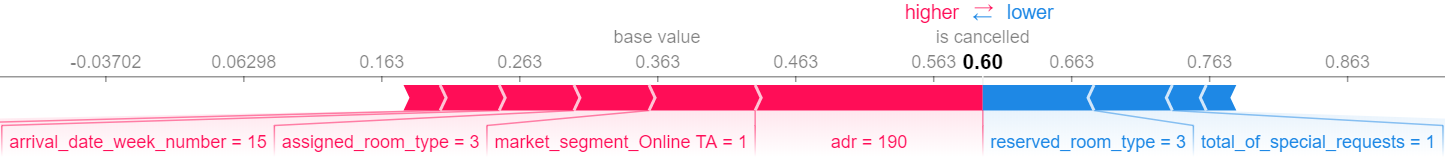
\includegraphics[width=\linewidth]{pics/myshap1.png}}
\end{figure}
\vspace{-2mm}

Все признаки, кроме market segment online TA, не совпадают с теми, что выявил LIME. Так как мы используем градиентный бустинг, имеет смысл попробовать TreeSHAP, так как он должен работать быстрее для нашей модели (но с меньшей точностью) -- он действительно рассчитал значения гораздо быстрее в сравнении с KernelSHAP:

\begin{figure}[h]
	\centering{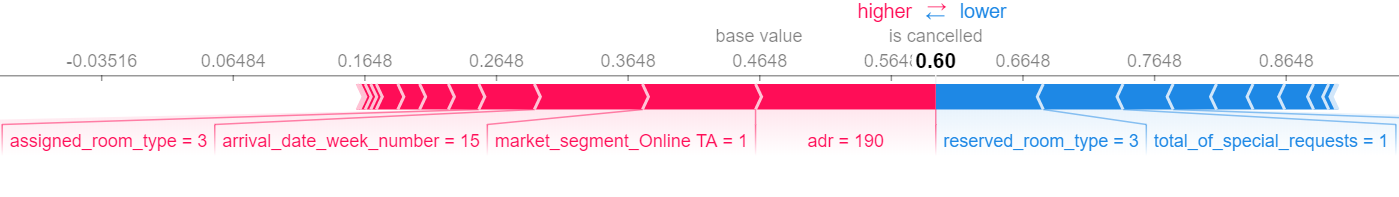
\includegraphics[width=\linewidth]{pics/myshap1t.png}}
\end{figure}
\vspace{-4mm}

Результат практически не поменялся: изменилась сила влияния некоторых признаков, assigned room type и arrival date week number поменялись местами -- TreeSHAP довольно-таки качественная замена KernelSHAP для моделей, основанных на деревьях. Остальные графики также практически не поменялись.

По обоим графикам можно сделать примерно одинаковые выводы. С точки зрения SHAP тип зарезервированной комнаты и дополнительные требования от клиента уменьшили вероятность того, что он отменит бронь. Тип комнаты представлен в зашифрованном виде, поэтому мы не можем сказать, корректно ли модель учитывает признак. Однако наличие дополнительных требований интерпретируется логично, так как предоставление необходимых клиенту услуг безусловно вызывает положительный отклик с его стороны.

В то же время такие признаки, как расходы, связанные с проживанием, бронь через онлайн-туроператора, неделя прибытия и предоставляемый тип комнаты (который будет предоставлен клиенту по факту -- может отличаться по техническим причинам или по желанию клиента). Первые два обсуждались ранее и интуитивно понятны. Последний также можно опустить, поскольку мы не знаем, как расшифровать признак. Стоит отметить, что забронированный и назначенный тип комнаты совпали -- требование клиента было выполнено. Соответственно, это должно снижать вероятность отмены. Но модель этого не учитывает, так как не знает взаимосвязи между признаками. В частности поэтому предикторы, связанные с типами комнаты, могли некорректно влиять на предсказание.

Мы рассмотрели отдельное предсказание. Попробуем также построить другие типы графиков, чтобы увидеть более общую картину -- возьмем подвыборку из 200 наблюдений.

\begin{figure}[h]
	\centering{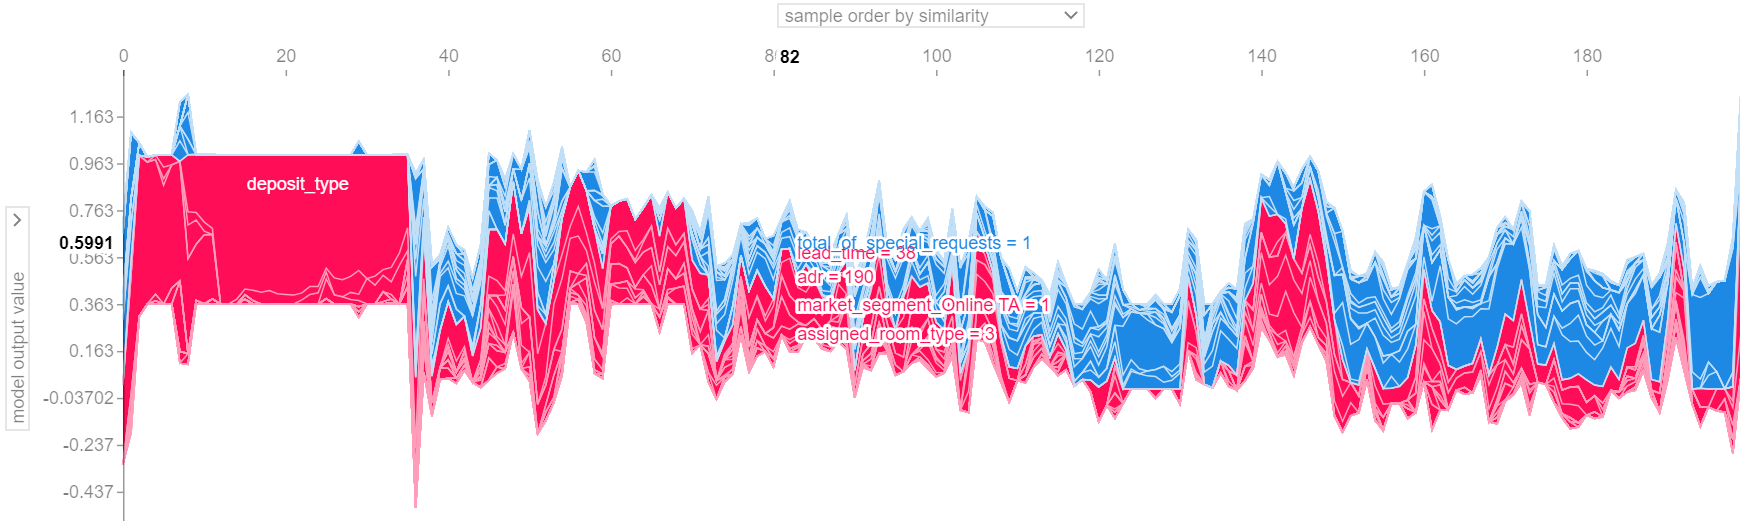
\includegraphics[width=\linewidth]{pics/myshap2.png}}
	\caption*{Forceplot для подвыборки: показывает, как получено предсказание для разных объектов}
\end{figure}

Данный график соединяет в себе индивидуальные графики для объектов выборки. По оси абсцисс отложены объекты из выборки, то есть мы можем одновременно смотреть на то, как сформировалось предсказание для разных наблюдений. Например, на графике отмечен объект, который мы уже рассматривали ранее, а также наиболее важные для его предсказания признаки.

Интерактивный интерфейс позволяет посмотреть различные комбинации. На графике выше показана зависимость предсказания модели от объекта, причем объекты были упорядочены по схожести между собой. Отсортируем объекты по значению предсказания:

\begin{figure}[h]
	\centering{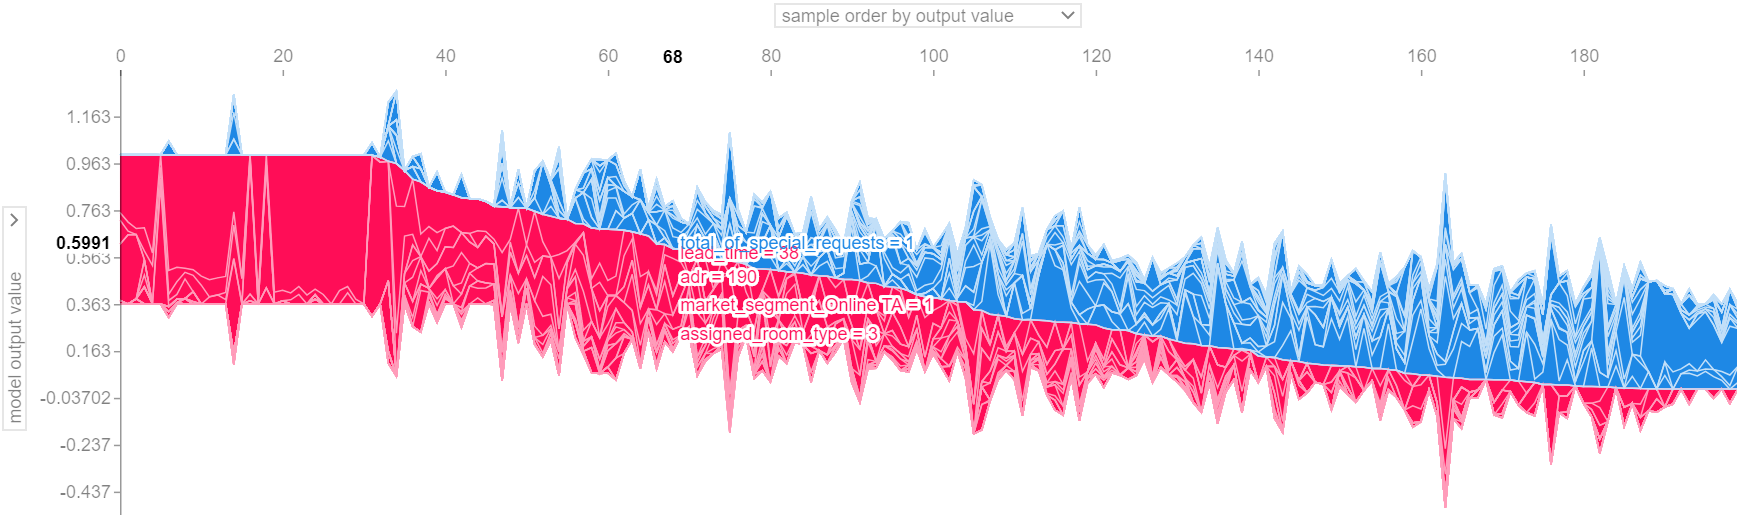
\includegraphics[width=\linewidth]{pics/myshap3.png}}
	\caption*{Forceplot: объекты отсортированы по значению предсказания}
\end{figure}

Наш объект переместился к началу координат. Также можно заметить наблюдения, для которых модель, <<по мнению SHAP>>, сделала уверенное предсказание -- вероятность примерно равна 1.

\vspace{-1mm}
\begin{figure}[h]
	\centering{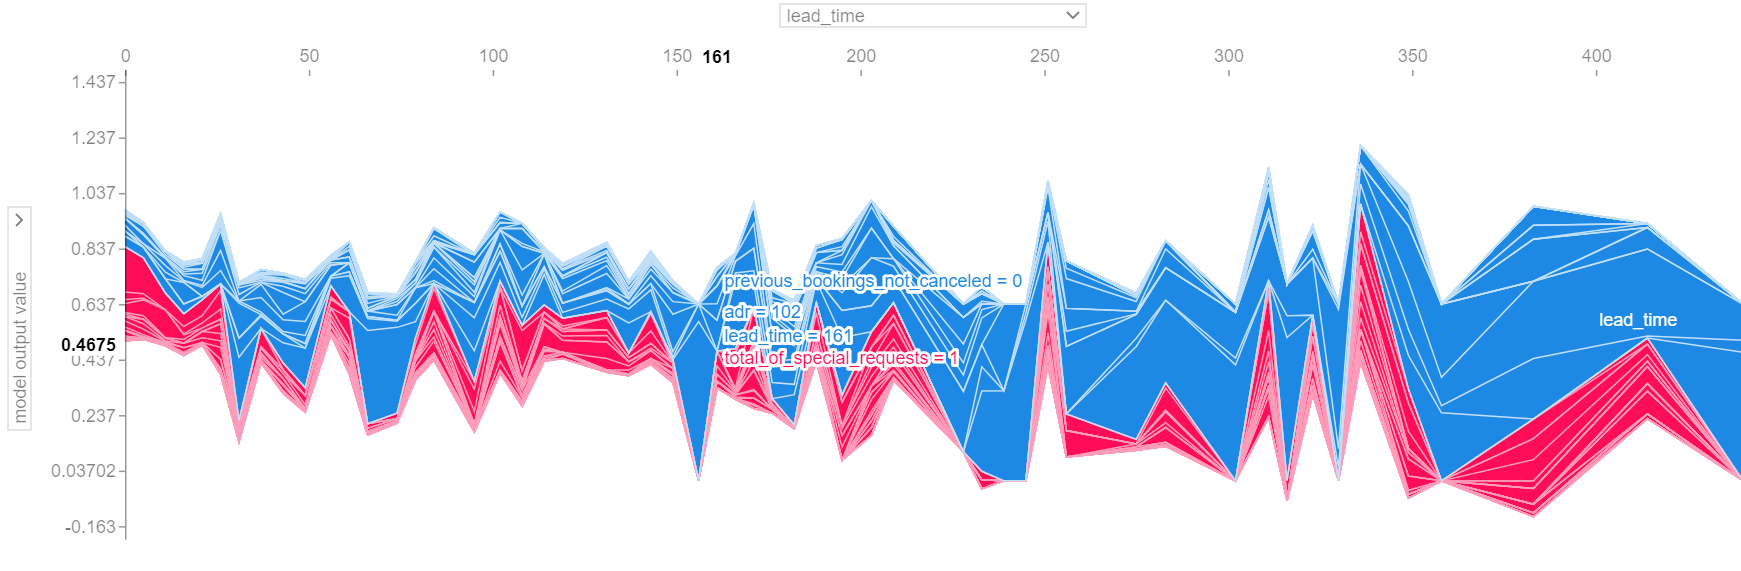
\includegraphics[width=\linewidth]{pics/myshap4.png}}
	\caption*{Forceplot: объекты отсортированы по возрастанию признака lead\_time}
\end{figure}
\vspace{-4mm}

Данный график является аналогом PDP, построенным по методу SHAP -- он показывает, как в среднем меняется предсказание в зависимости от значения признака lead time. Но поскольку влияние предикторов в PDP и SHAP рассчитывается разными способами, графики оказались не слишком похожи.

\vspace{-1mm}
\begin{figure}[h]
	\centering{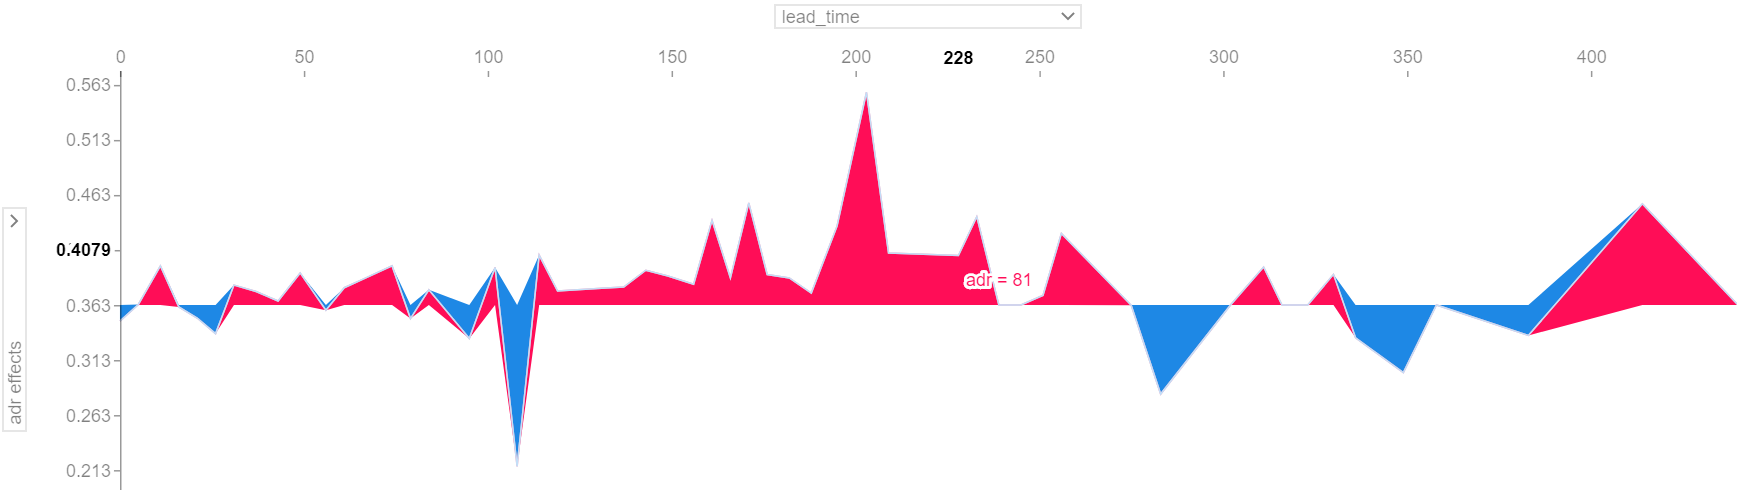
\includegraphics[width=\linewidth]{pics/myshap5.png}}
	\caption*{Forceplot: зависимость эффектов признака adr от признака lead\_time}
\end{figure}
\vspace{-4mm}

Также можно посмотреть, как меняется эффект от выбранного признака при разных значениях другого -- некоторый аналог PDP для двух признаков. Например, при adr = 81 lead time увеличивает вероятность отмены

\begin{tabular}{c|c}
	\arrayrulecolor[rgb]{0.8,0.85,1}
	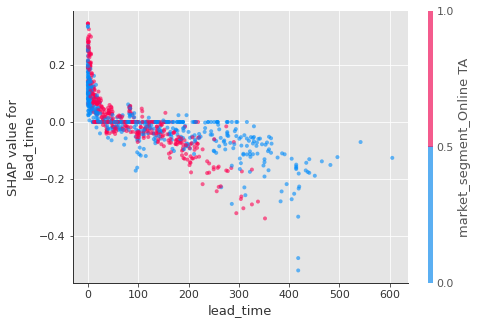
\includegraphics[width=0.47\linewidth]{pics/myshap6.png} & 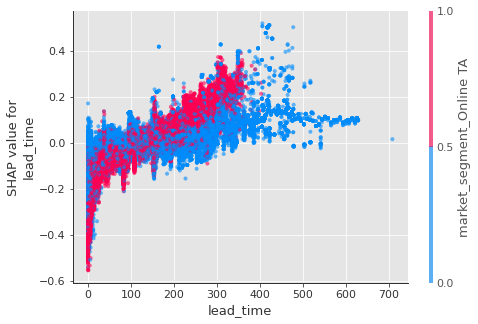
\includegraphics[width=0.47\linewidth]{pics/myshap6t.png} \\
	KernelSHAP & TreeSHAP \\
\end{tabular}\\[-6mm]
\begin{center}
	Dependence plot для признака: зависимость SHAP value признака от его значения
\end{center}
\vspace{-3mm}

Данный тип графика значительно отличается для выбранных методов. Для KernelSHAP график был построен по подвыборке из 200 объектов, для TreeSHAP по всей выборке.

По левому графику можно сделать вывод, что чем меньше значение lead time, тем более значим признак для предсказания. Интересно, что, например, при lead time $=100$ SHAP~value, то есть вклад признака в предсказание, может быть как положительным, так и отрицательным. Цвет точек на графике показывает значение другого признака, в данном случае market segment online TA -- он выбирается автоматически, как признак с которым выбранный взаимодействует сильнее всего. Зависимость, показанная на графике, может быть разной для разных значений признака market segment online TA -- для красных точек зависимость более сильная, чем для голубых.

Для правого графика получаются противоположные выводы, так как зависимость стала ровно обратной. Данная ситуация может быть связана с погрешностью метода TreeSHAP.

\noindent
\begin{tabular}{cc}
	\arrayrulecolor[rgb]{0.8,0.85,1}
	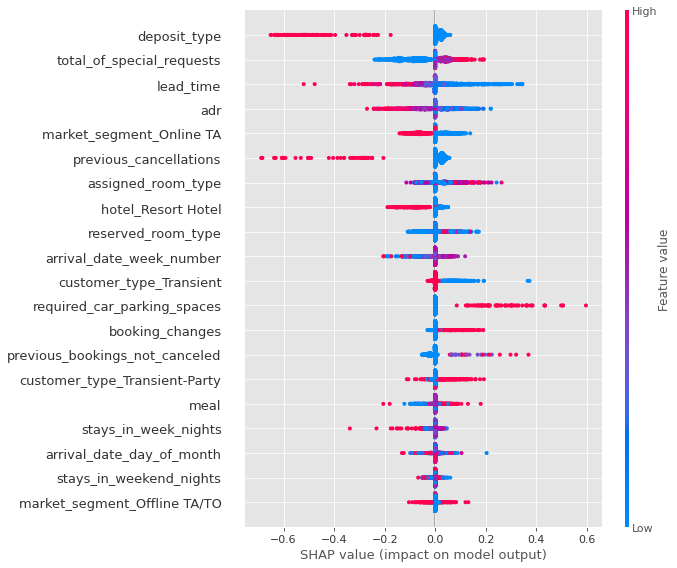
\includegraphics[width=0.61\linewidth]{pics/myshap7.png} & 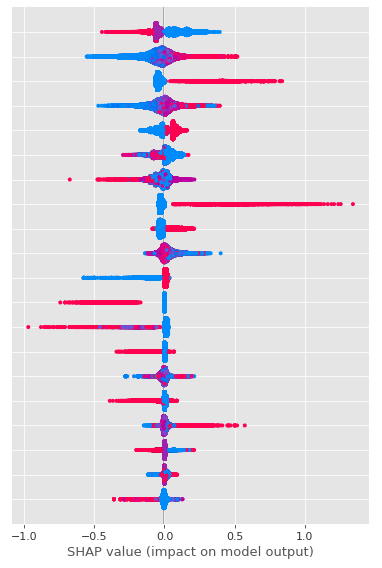
\includegraphics[width=0.34\linewidth]{pics/myshap7t.png} \\
	KernelSHAP & TreeSHAP \\
\end{tabular}\\[-5mm]
\begin{center}
	Summary plot для всех признаков и объектов: показывает выборочное распределение признаков, их SHAP values
\end{center}
\vspace{-3mm}

Исходя из названия графика: он показывает некоторую сводку по предикторам и их важности для модели. По вертикали расположены разные признаки, по горизонтали их SHAP value, цвет точек определяет значение признака. Графики для разных методов SHAP отличаются.

Некоторые выводы:\\[-8mm]
\begin{itemize}
	\item влияние total special requests равномерно распределяется: при высоких значениях -- большой отрицательный вклад, при низких значениях -- большой положительный вклад. Но для многих объектов он оказался незначительным\\[-7mm]
	\item для KernelSHAP: required car parking spaces не вносит вклад при маленьких значениях (0), и вносит большой положительный вклад в предсказание при больших значениях. Для TreeSHAP: наоборот\\[-7mm]
\end{itemize}

Сложилась странная ситуация, в которой два метода SHAP противоречат друг другу. Это может быть связано с тем, что для KernelSHAP мы использовали подвыборку вместо всей выборки, с погрешностью TreeSHAP при расчете значений Шэпли и т.д. Это еще раз подтверждает мысль о том, что необходимо с осторожностью относиться к данным методам интерпретации

SHAP дает более детальную картину. Мы можем посмотреть как на отдельное предсказание, так и на глобальное влияние признака. Он сочетает в себе достоинства PDP и LIME. Однако к его результатам стоит относиться аккуратно, так же, как это было с другими методами. При интерпретации стоит рассматривать ситуацию с разных сторон, строить больше графиков, чтобы убедиться в некоторой зависимости.
	\newpage
	
	\section{Заключение}
	Мы рассмотрели три метода интерпретации моделей машинного обучения: PDP, LIME, SHAP. Они имеют довольно-таки строгое математическое обоснование: простые, но красивые идеи, которые нашли свое применение в машинном обучении. Важным общим свойством методов является использование графиков и картинок -- наиболее понятная, хорошо интерпретируемая человеком форма информации.

Существует огромное количество других методов, помимо приведенных, которые также хорошо интерпретируют работу модели. В последнее время данная область развивается особенно активно, так как распространение использования машинного обучения вызвало рост спроса на объяснение и интерпретацию результатов разных техник. 

Описанные методы позволяют интерпретировать результат работы любой модели. Это полезное средство для самых разных исследований. Как мы уже заметили, они имеют свои недостатки, не всегда точно показывают влияние признаков на предсказание. Тем не менее они выполняют основную задачу -- представляют результат работы модели в понятном человеку виде.
	\newpage
	
	\begin{thebibliography}{99}
		\bibitem{basis}
		\href{https://christophm.github.io/interpretable-ml-book/}{Interpretable Machine Learning | Christoph Molnar | Christoph Molnar | 2020 | ch. 1, 2, 5}
		\bibitem{pdpgit}
		\href{https://github.com/SauceCat/PDPbox}{PDPbox | Li Jiangchun (SauceCat) | GitHub}
		\bibitem{pdp}
		\href{https://www.cse.cuhk.edu.hk/irwin.king/_media/presentations/2001_greedy_function_approximation_a_gradient_boosting_machine.pdf}{Greedy Function Approximation: a Gradient Boosting Machine} | Jerome H. Friedman | 1999 | p. 1219-1220
		\bibitem{lime_dop}
		\href{https://pbiecek.github.io/ema/LIME.html}{Explanatory Model Analysis} | Przemyslaw Biecek, Tomasz Burzykowski | 2020 | ch. 10
		\bibitem{limegit}
		\href{https://github.com/marcotcr/lime}{LIME | Marco Tulio Correia Ribeiro (marcotcr) | GitHub}
		\bibitem{lime}
		\href{https://arxiv.org/pdf/1602.04938.pdf}{“Why Should I Trust You?” Explaining the Predictions of Any Classifier} | Marco Tulio Ribeiro, Sameer Singh, Carlos Guestrin | 2016 | p. 3-6
		\bibitem{shap}
		\href{https://arxiv.org/pdf/1705.07874.pdf}{A Unified Approach to Interpreting Model Predictions} | Scott M. Lundberg, Su-In Lee | 2017 | p. 3-7
		\bibitem{shapgit}
		\href{https://github.com/slundberg/shap}{SHAP | Scott Lundberg (slundberg) | GutHub}
		\bibitem{data}
		\href{https://www.kaggle.com/jessemostipak/hotel-booking-demand}{Hotel booking demand | Kaggle}
		\bibitem{pdptut}
		\href{https://pdpbox.readthedocs.io/en/latest/}{PDPbox tutorial}
		\bibitem{linetut}
		\href{https://lime-ml.readthedocs.io/en/latest/}{LIME tutorial}
		\bibitem{shaptut}
		\href{https://shap.readthedocs.io/en/latest/}{SHAP tutorial}
		\bibitem{dop1}
		\href{https://towardsdatascience.com/interpretable-machine-learning-1dec0f2f3e6b}{Interpretable Machine Learning} | Parul Pandey | Medium | 2019
		\bibitem{dop2}
		\href{https://arxiv.org/pdf/1802.03888.pdf}{Consistent Individualized Feature Attribution for Tree Ensembles} | Scott M. Lundberg, Gabriel G. Erion, and Su-In Lee | 2019 | p. 1-4
	\end{thebibliography}
	\newpage
\end{document}